This category of backgrounds includes processes with a single leptonic \W~decay, giving rise to one lepton and \met\ from a single neutrino.
As a result, the \mt\ variable, constructed from the lepton and the \met, exhibits a kinematic edge at $\mt \sim \mW$. The main contributors
to this background are \ttlj, \wjets\ and single top, though in the latter case there is a contribution from \tw\ that can give rise to two leptons. 
The 2-lepton single top background is included in the rare backgrounds estimate. 

\subsubsection{W+Jets MC Modelling Validation}

The estimate of the uncertainty on this background is based on CR1, 
defined by applying the full signal selection, but requiring 0 b-tags. 
The sample is dominanted by \wjets\ and is thus used to validate the MC modelling of this background. 

\begin{table}[!h]
\begin{center}
\begin{tabular}{l||c||c|c|c|c}
\hline
Sample              & CR1PRESEL & CR1A & CR1B & CR1C & CR1D \\
\hline
\hline
Muon \mt-SF 	  & $0.91 \pm 0.03$ & $0.96 \pm 0.07$ & $0.88 \pm 0.11$ & $1.05 \pm 0.21$ & $1.27 \pm 0.41$ \\
\hline
\hline
Electron \mt-SF 	  & $0.82 \pm 0.03$ & $0.86 \pm 0.06$ & $1.09 \pm 0.15$ & $1.24 \pm 0.30$ & $1.11 \pm 0.40$ \\
\hline
\end{tabular}
\caption{ \mt\ peak Data/MC scale factors applied to the single lepton
  samples and \ttdl. The raw MC is used for backgrounds from rare
  processes. CR1PRESEL refers to a sample with $\met>50$ GeV.
  The uncertainties are statistical only.
\label{tab:cr1mtsf}}
\end{center}
\end{table}



\begin{table}[!h]
\begin{center}
\begin{tabular}{l||c||c|c|c|c}
\hline
Sample              & CR1PRESEL & CR1A & CR1B & CR1C & CR1D \\
\hline
\hline
Muon MC 		  & $456 \pm 73$ & $174 \pm 44$ & $51 \pm 7$ & $18 \pm 2$ & $10 \pm 2$ \\
Muon Data 		  & $657$ & $246$ & $142$ & $43$ & $12$ \\
\hline
Muon Data/MC SF 	  & $1.44 \pm 0.24$ & $1.41 \pm 0.37$ & $2.80 \pm 0.47$ & $2.37 \pm 0.46$ & $1.23 \pm 0.42$ \\
\hline
\hline
Electron MC 		  & $396 \pm 64$ & $147 \pm 36$ & $54 \pm 4$ & $19 \pm 2$ & $8 \pm 2$ \\
Electron Data 		  & $702$ & $223$ & $144$ & $50$ & $23$ \\
\hline
Electron Data/MC SF 	  & $1.77 \pm 0.29$ & $1.52 \pm 0.39$ & $2.68 \pm 0.30$ & $2.57 \pm 0.49$ & $2.73 \pm 0.76$ \\
\hline
\end{tabular}
\caption{ Yields in \mt\ tail comparing the MC prediction (after
  applying SFs) to data. CR1PRESEL refers to a sample with $\met>50$
  GeV and $\mt>150$ GeV.
  The uncertainties are statistical only.
\label{tab:cr1yields}}
\end{center}
\end{table}

\begin{figure}[hbt]
  \begin{center}
	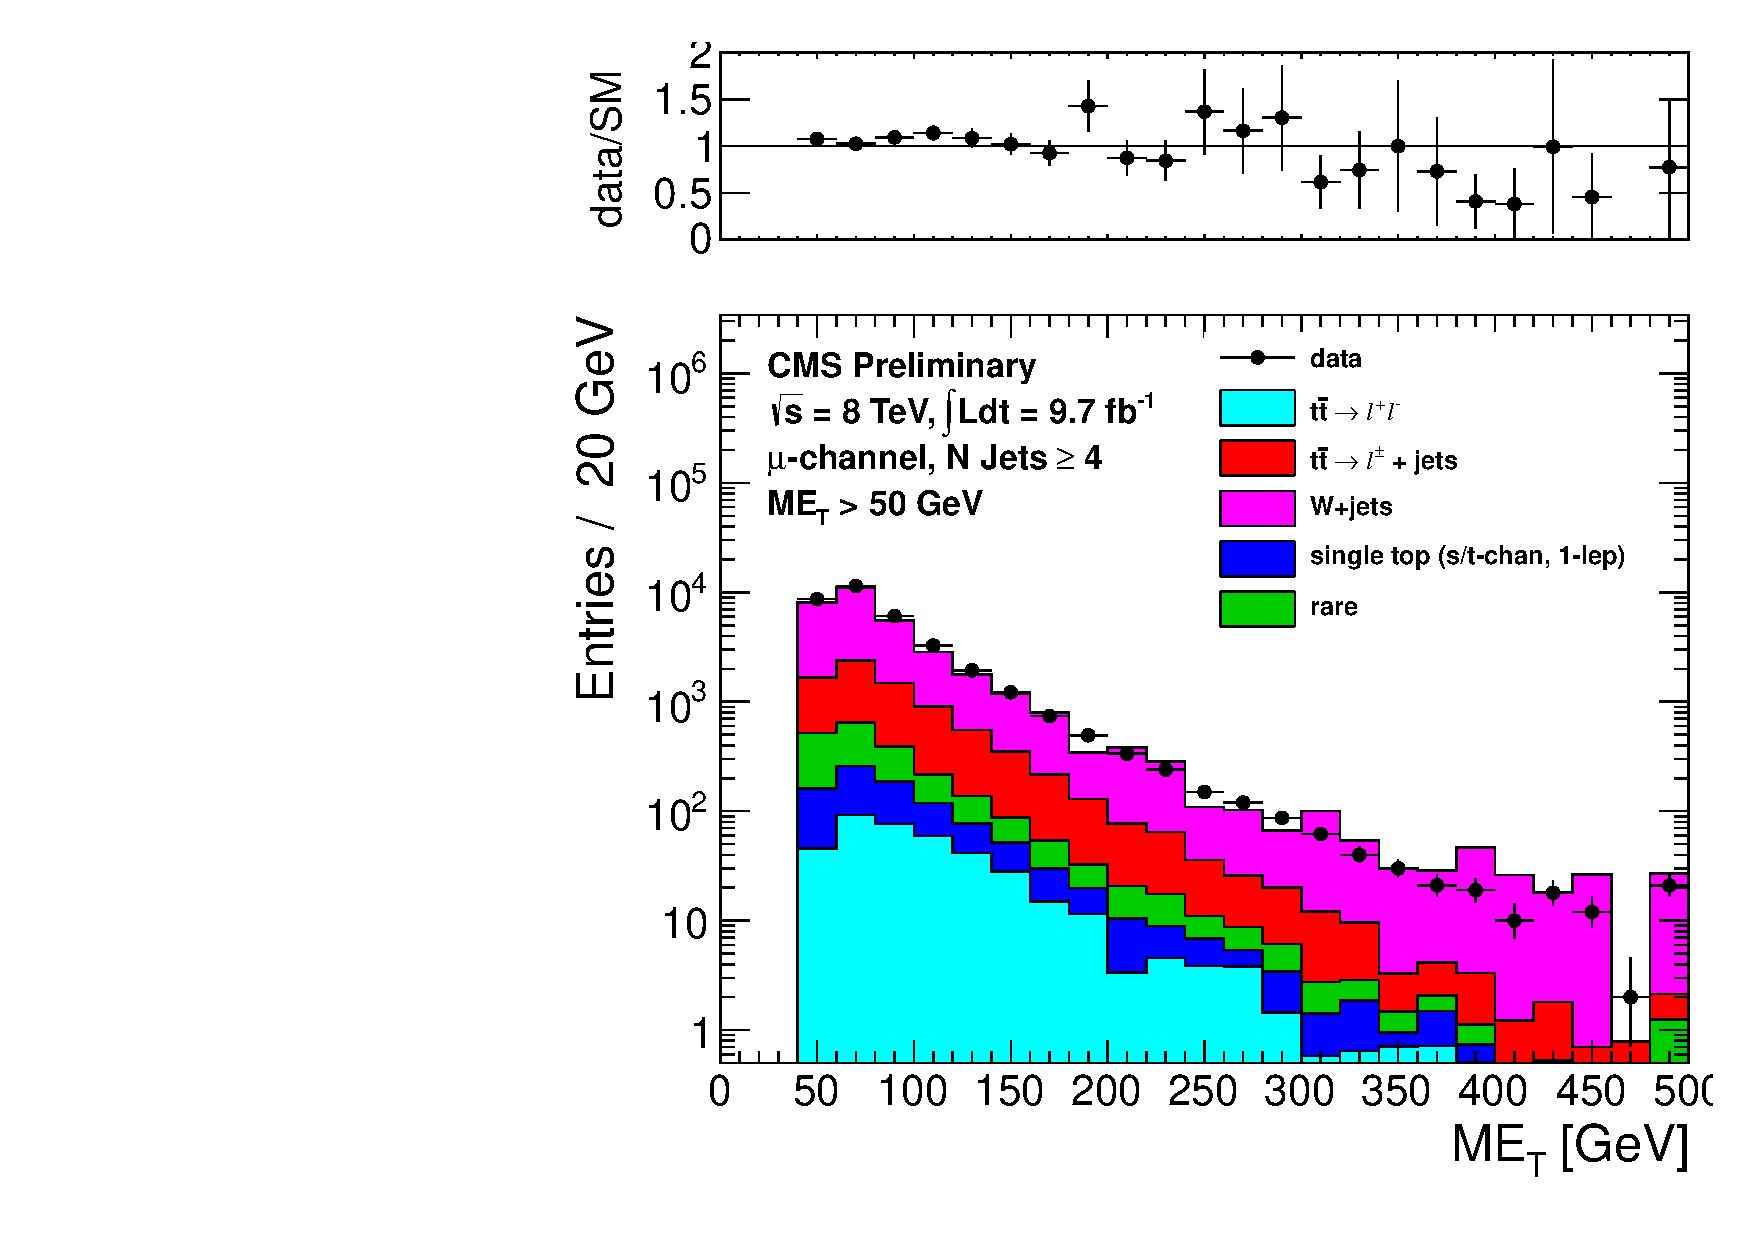
\includegraphics[width=0.5\linewidth]{plots/CR1plots/met_met50_leadmuo_nj4.pdf}%
	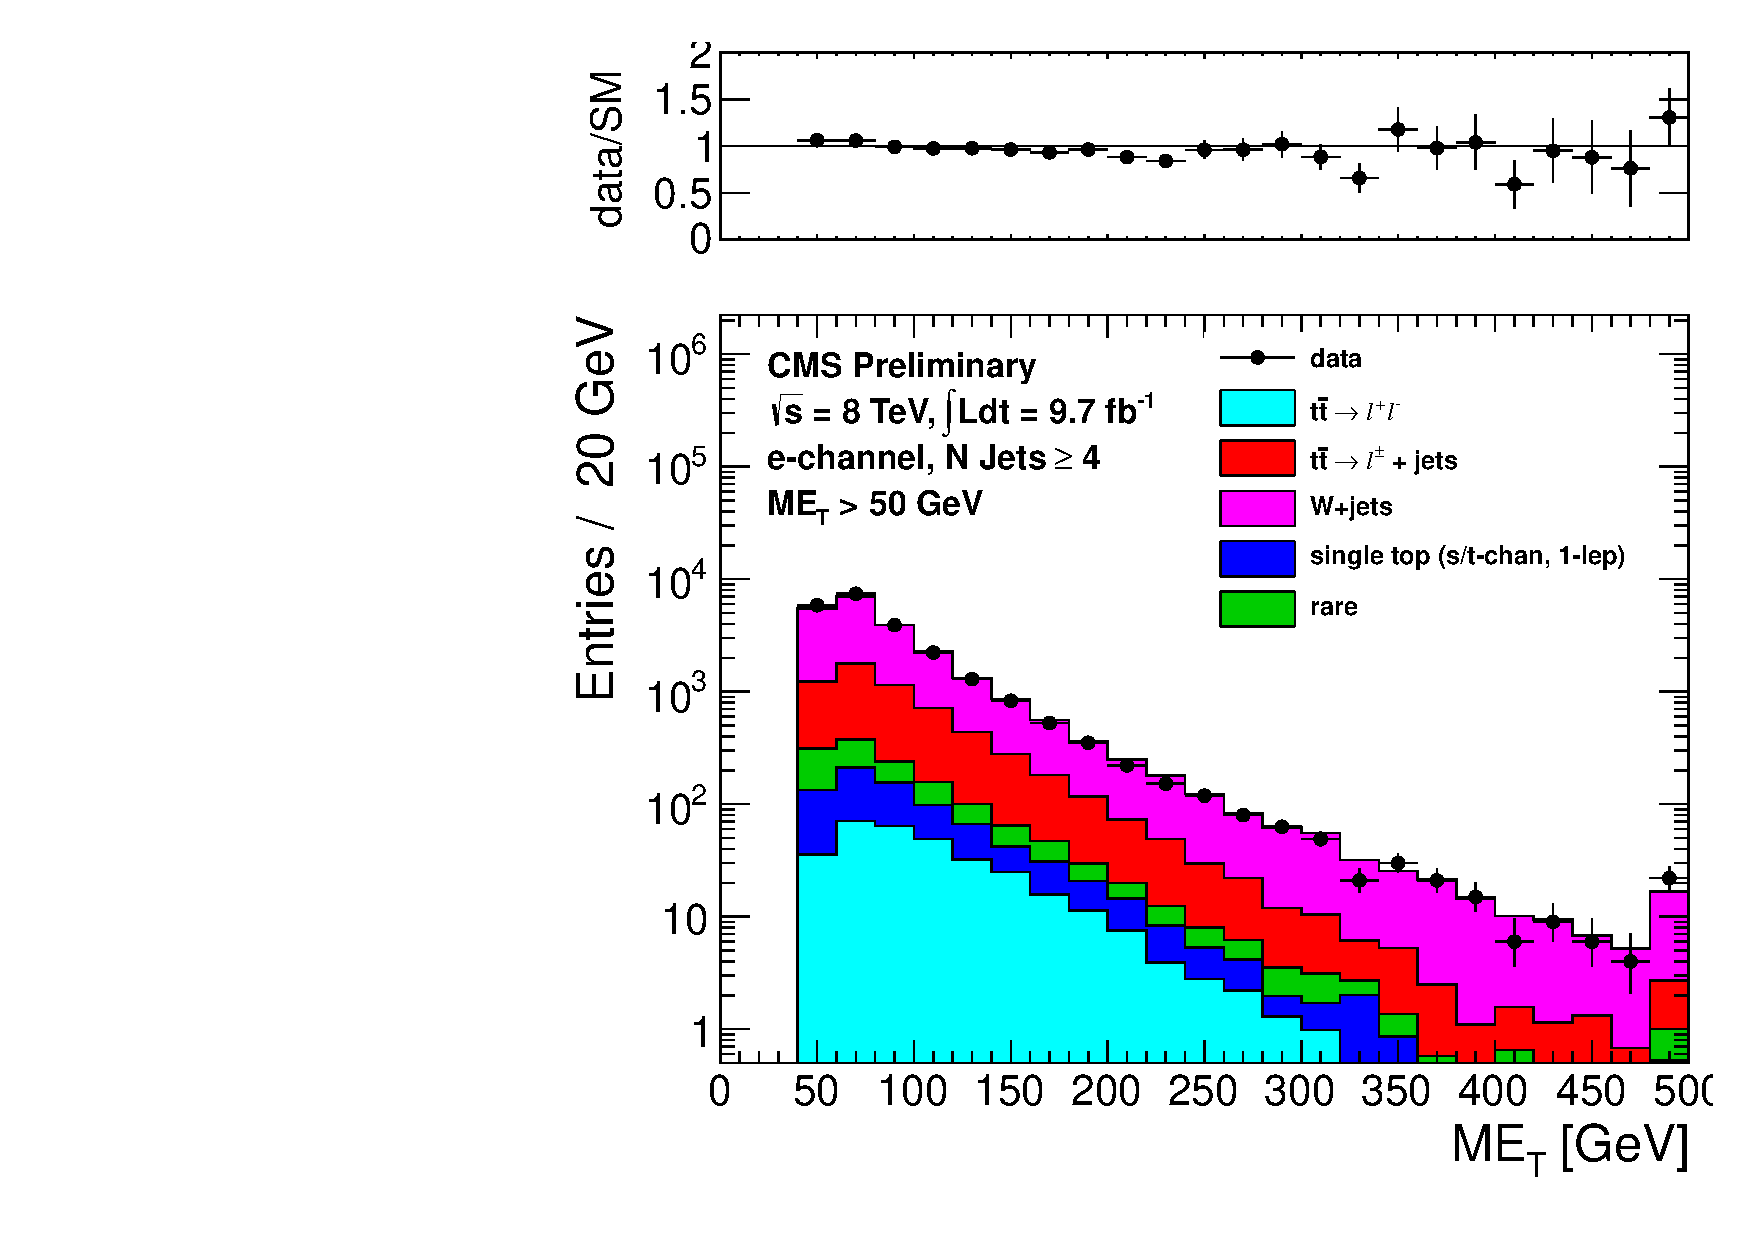
\includegraphics[width=0.5\linewidth]{plots/CR1plots/met_met50_leadele_nj4.pdf}
	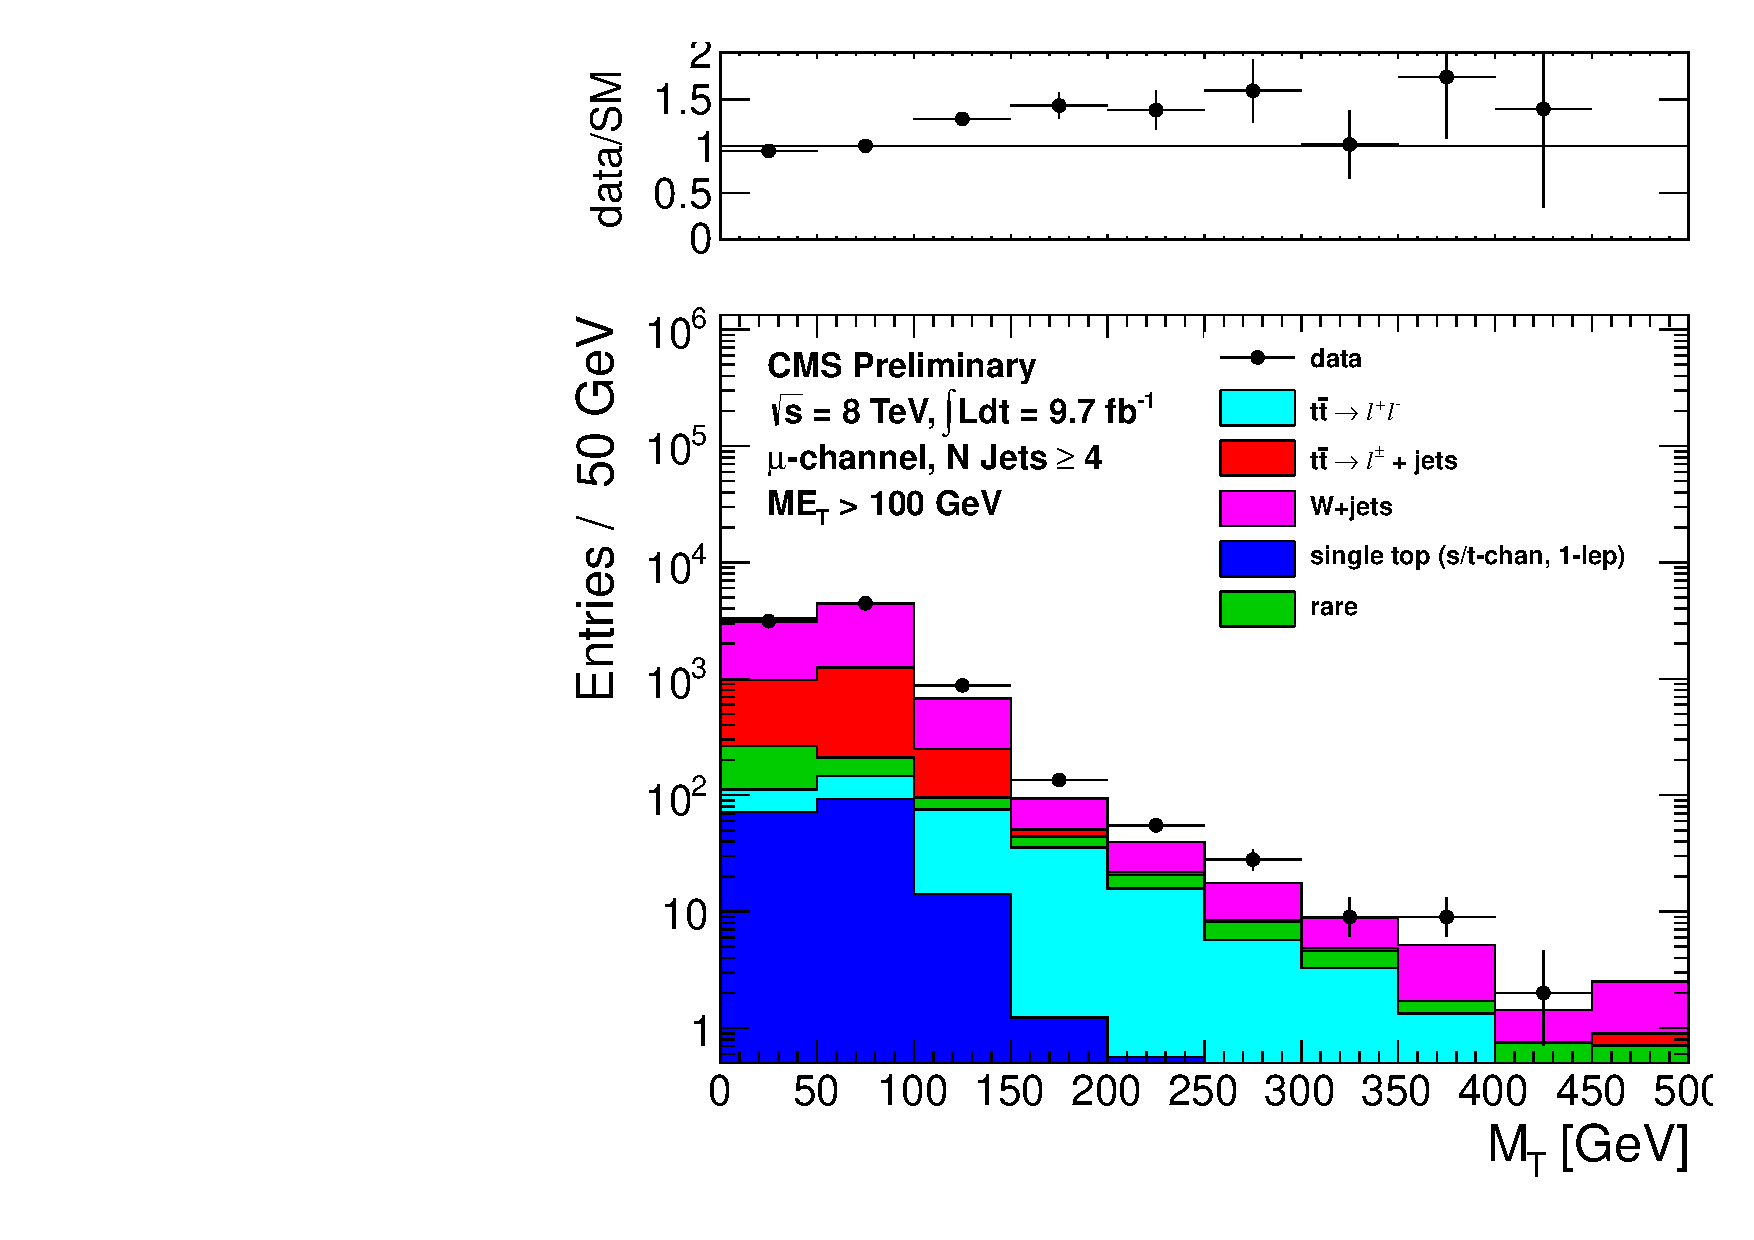
\includegraphics[width=0.5\linewidth]{plots/CR1plots/mt_met100_leadmuo_nj4.pdf}%
	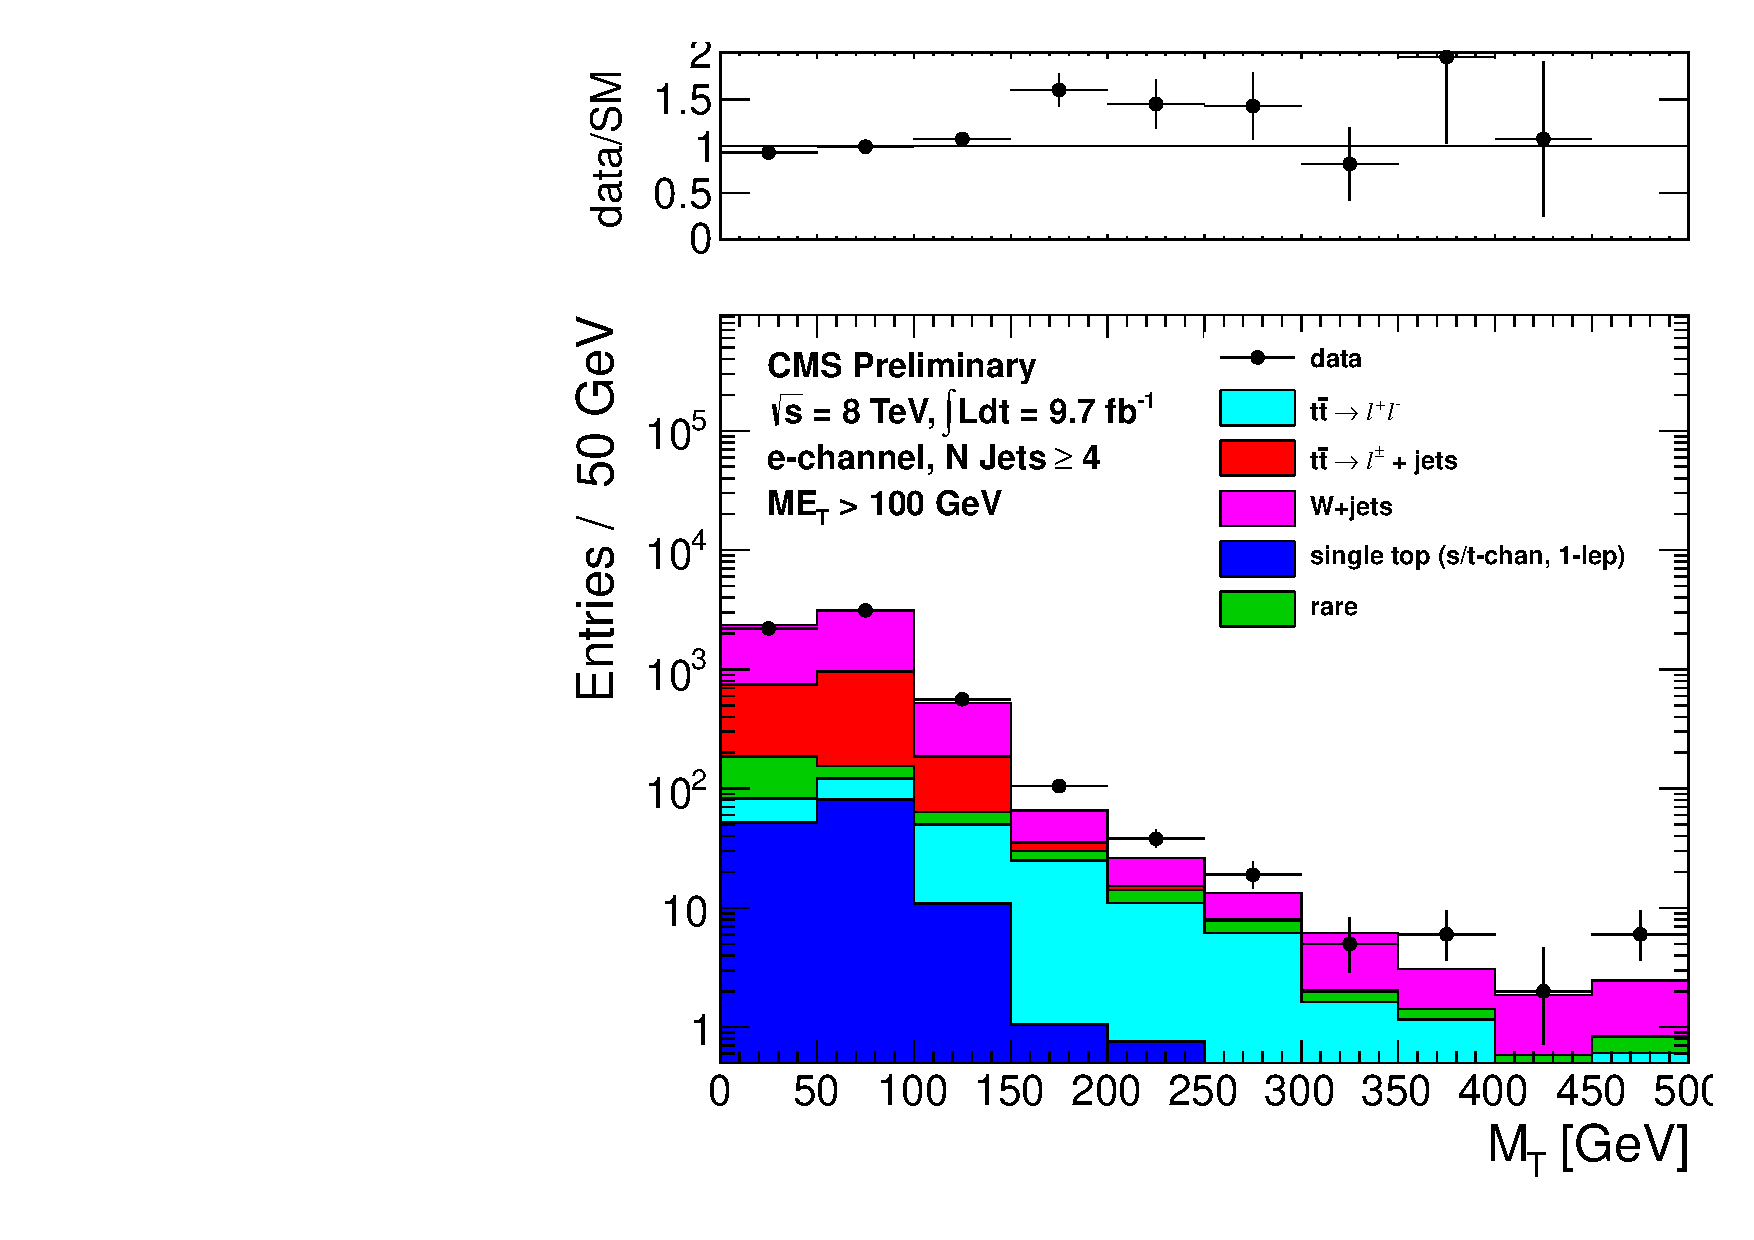
\includegraphics[width=0.5\linewidth]{plots/CR1plots/mt_met100_leadele_nj4.pdf}
    \caption{
      Comparison of the \met\ (top) and \mt\ for $\met>100$ (bottom) distributions in data vs. MC for events
      with a leading muon (left) and leading electron (right)
      satisfying the requirements of CR1. 
\label{fig:cr1met} 
}  
      \end{center}
\end{figure}

\begin{figure}[hbt]
  \begin{center}
	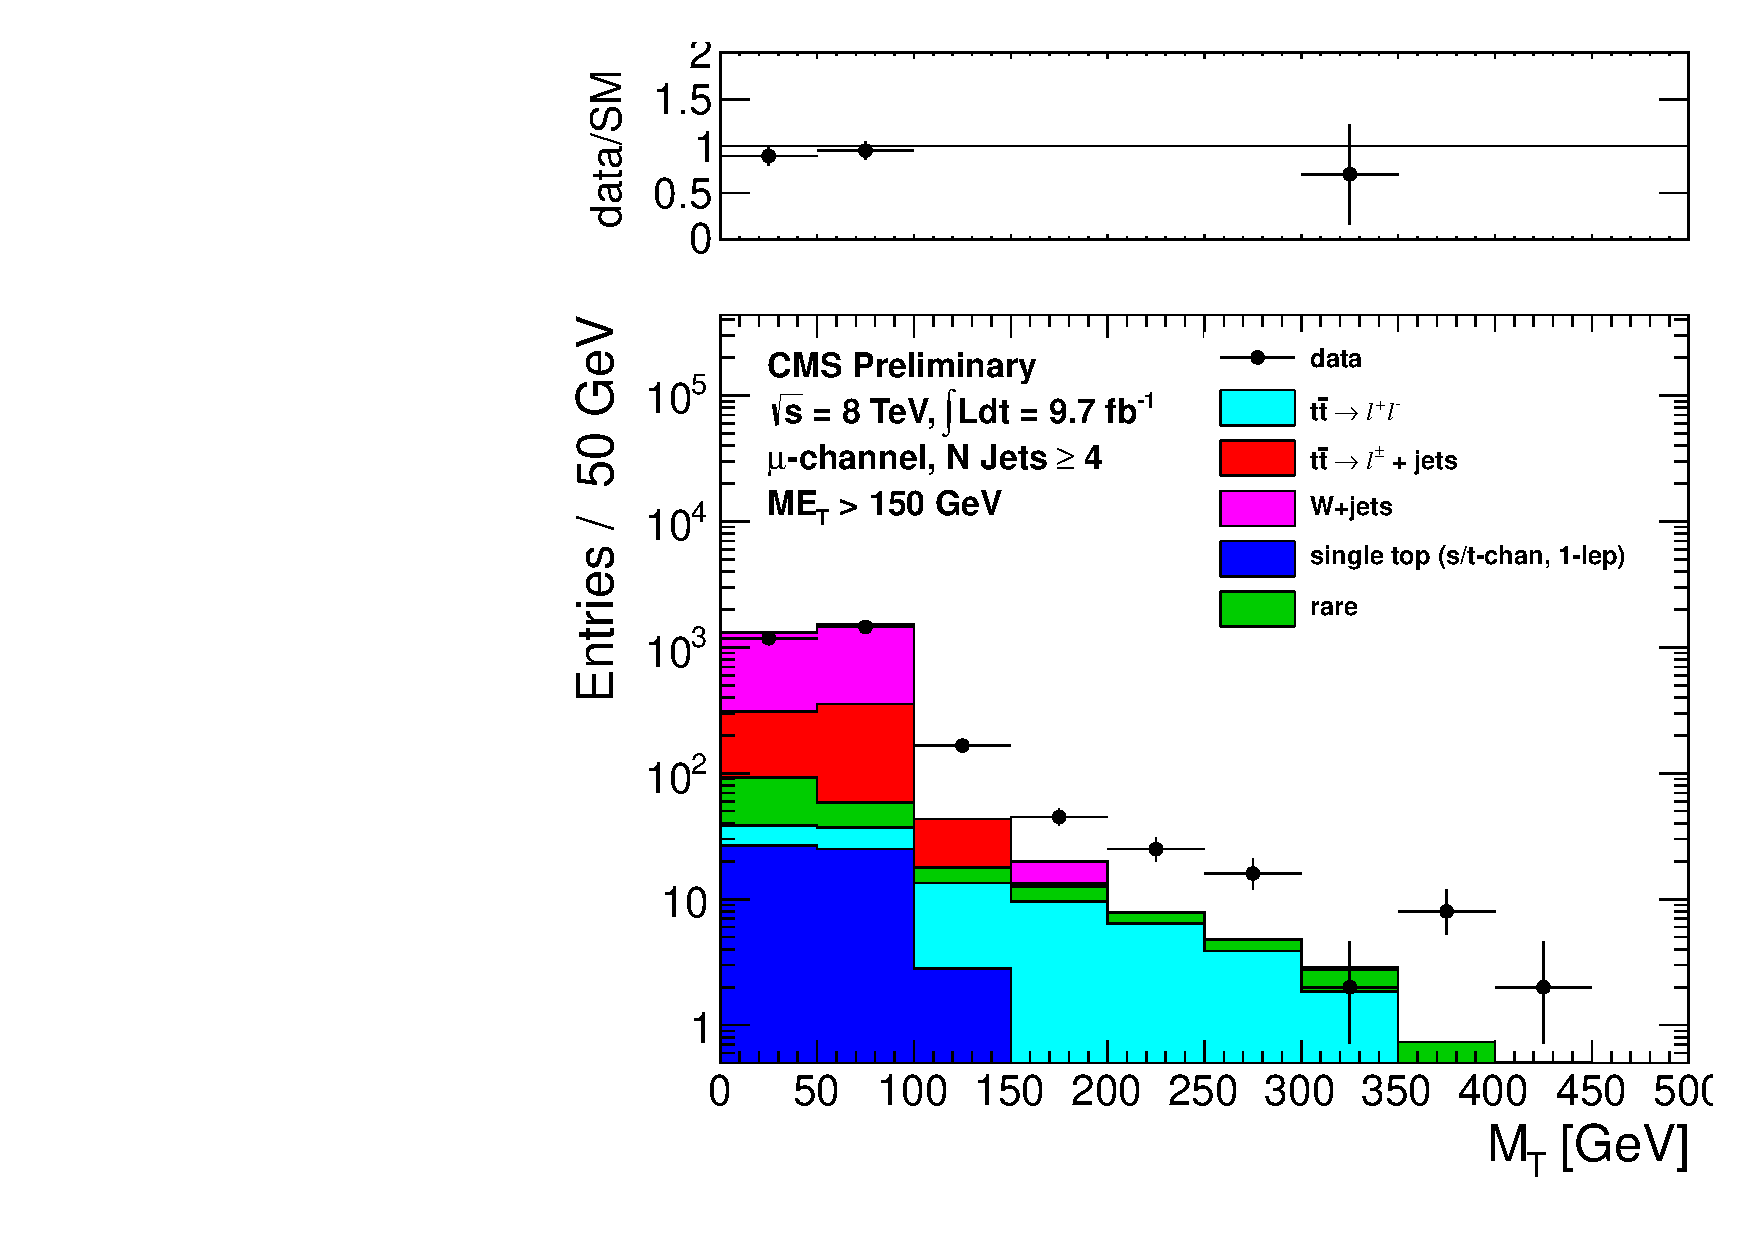
\includegraphics[width=0.5\linewidth]{plots/CR1plots/mt_met150_leadmuo_nj4.pdf}%
	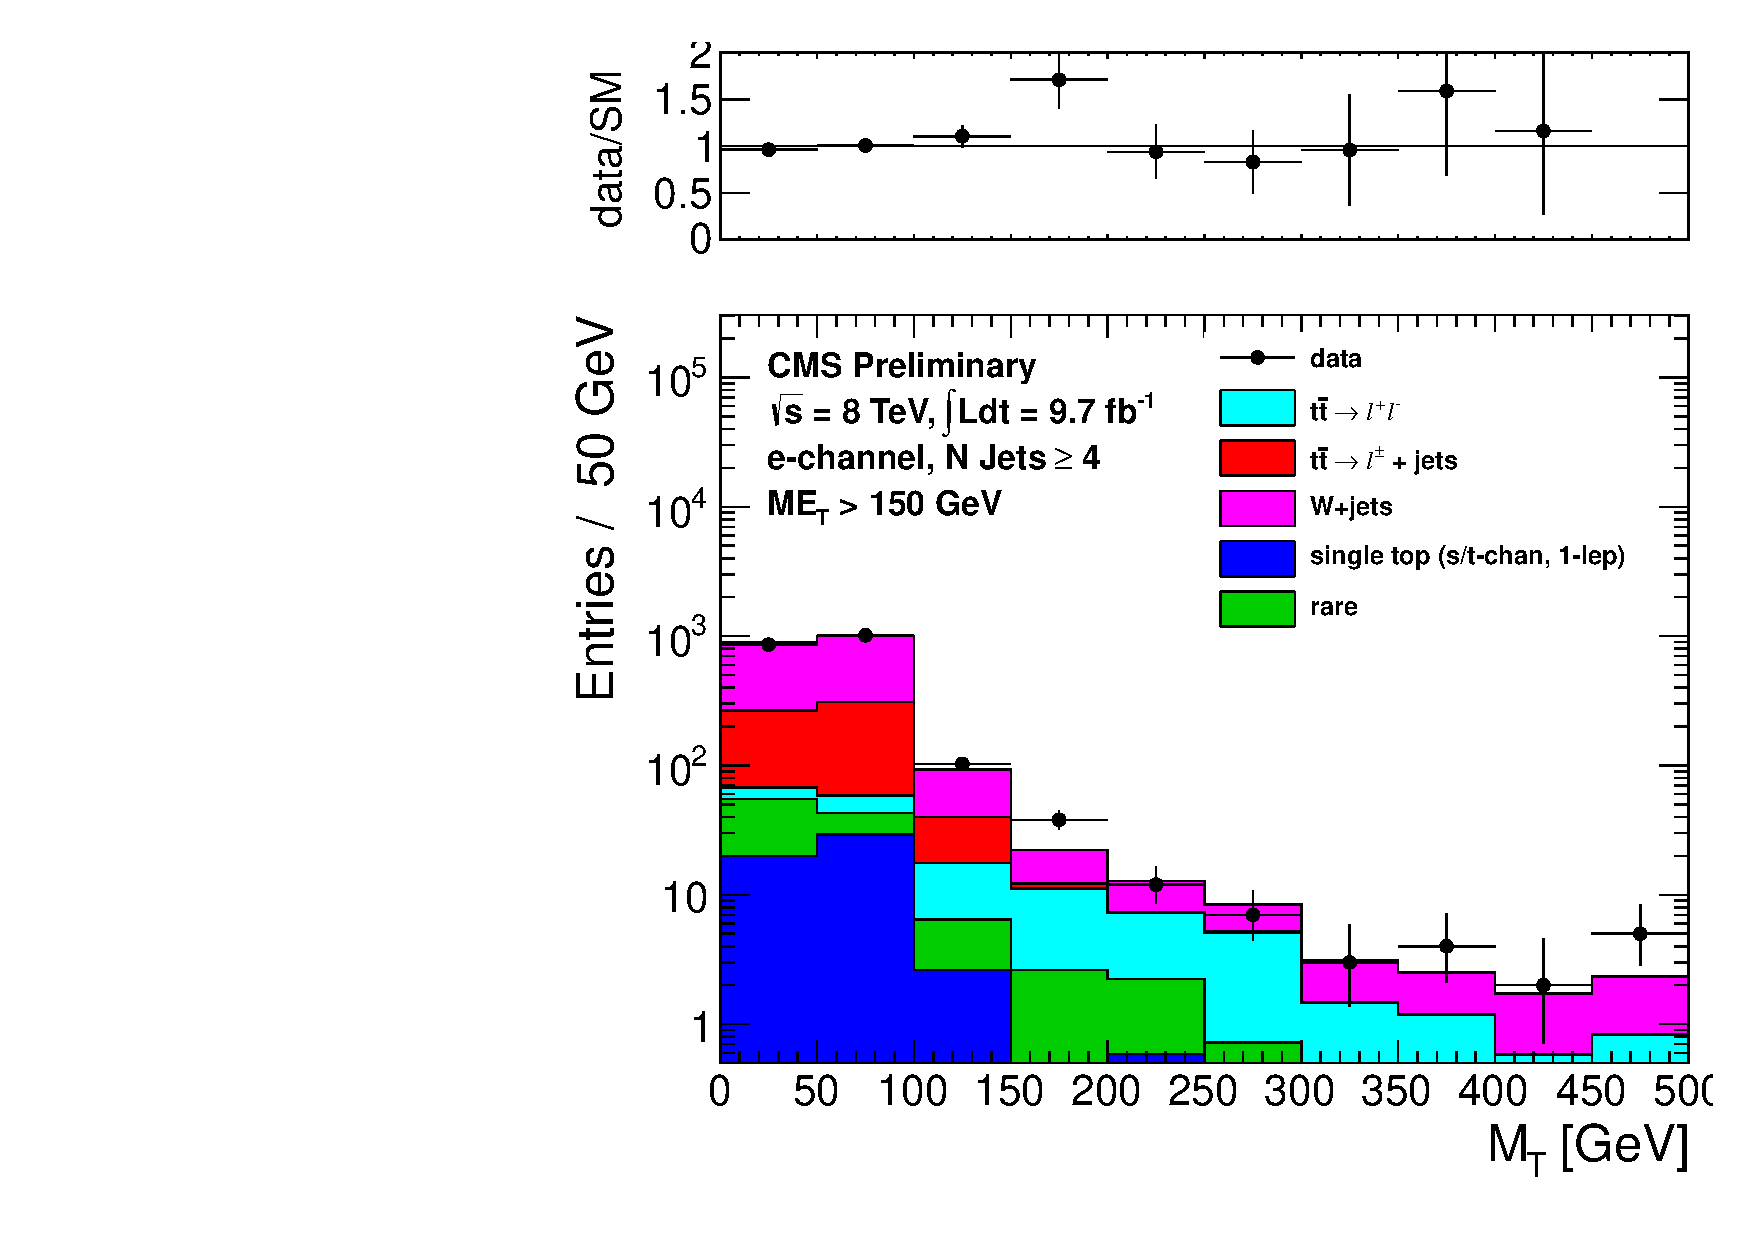
\includegraphics[width=0.5\linewidth]{plots/CR1plots/mt_met150_leadele_nj4.pdf}
	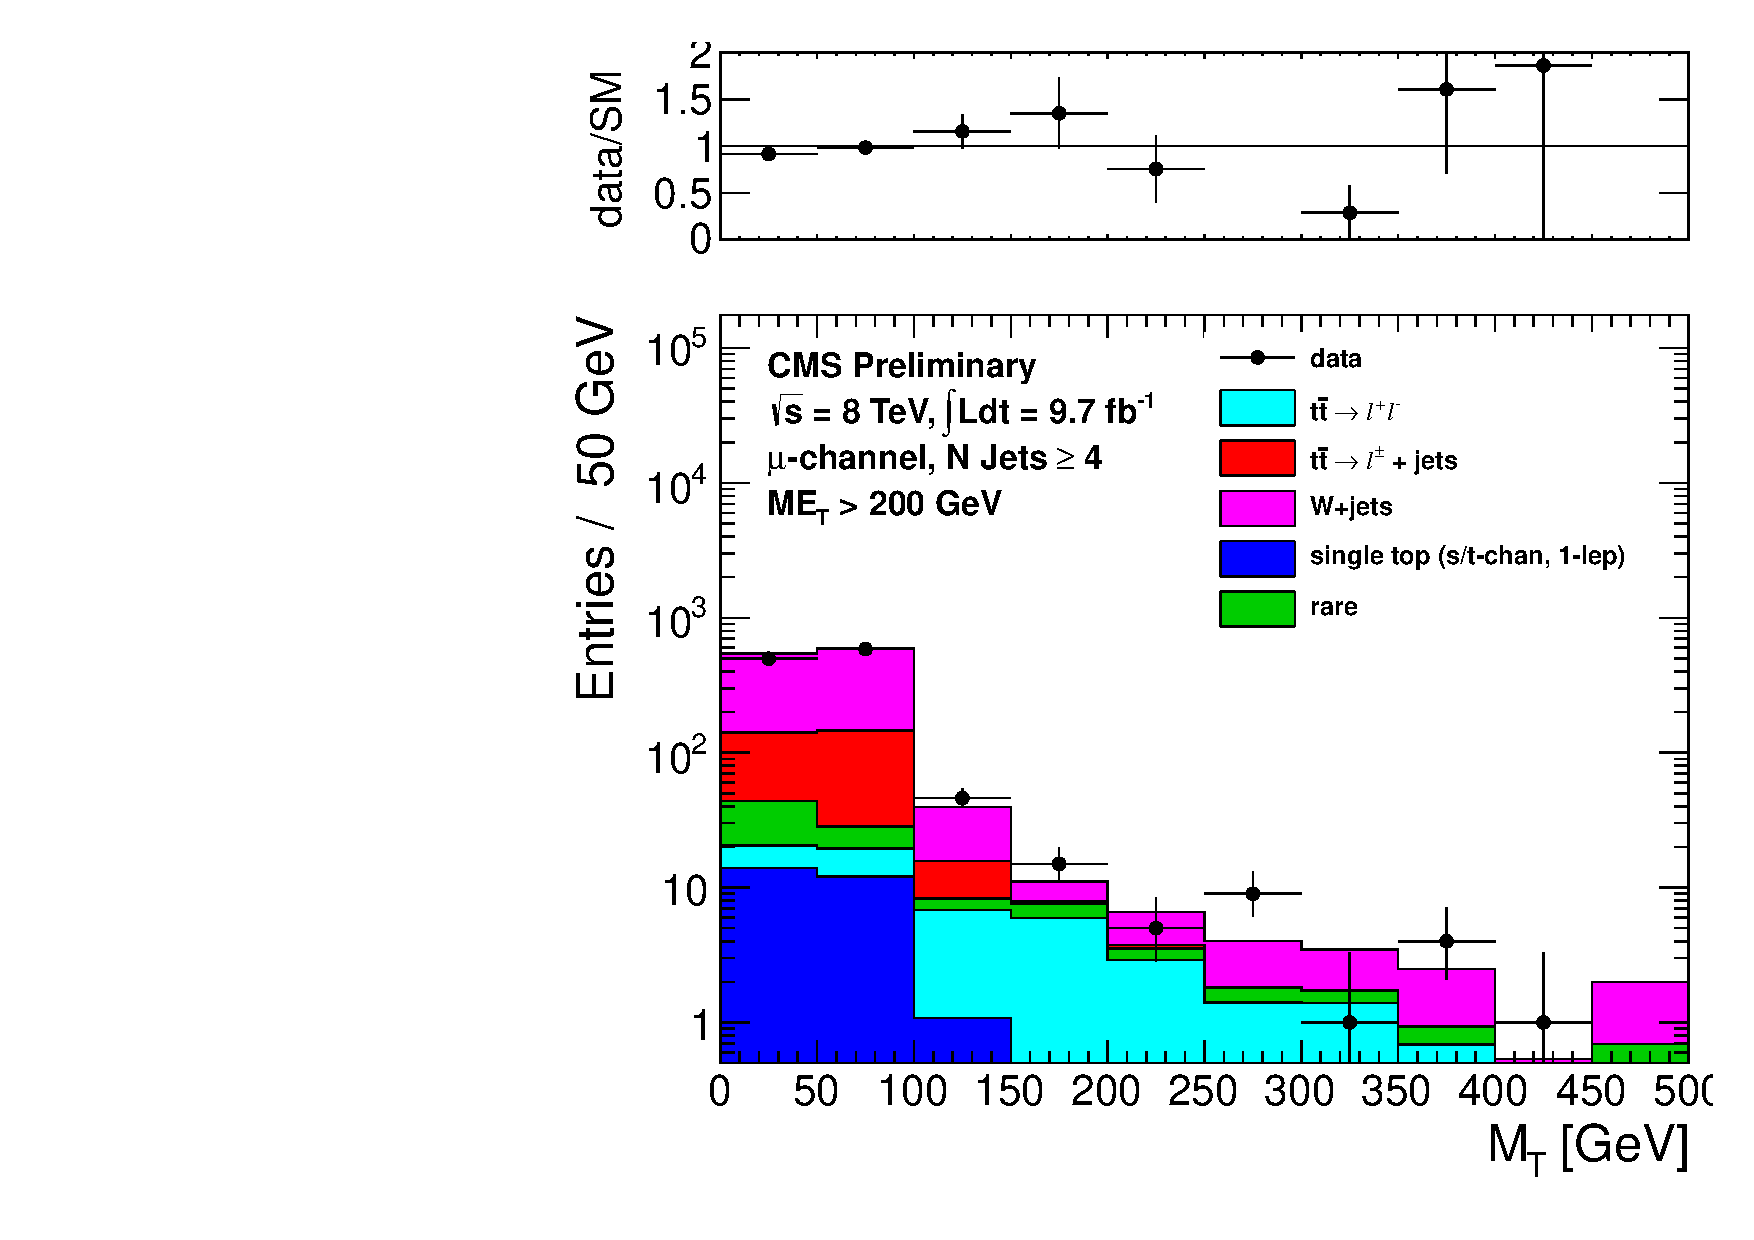
\includegraphics[width=0.5\linewidth]{plots/CR1plots/mt_met200_leadmuo_nj4.pdf}%
	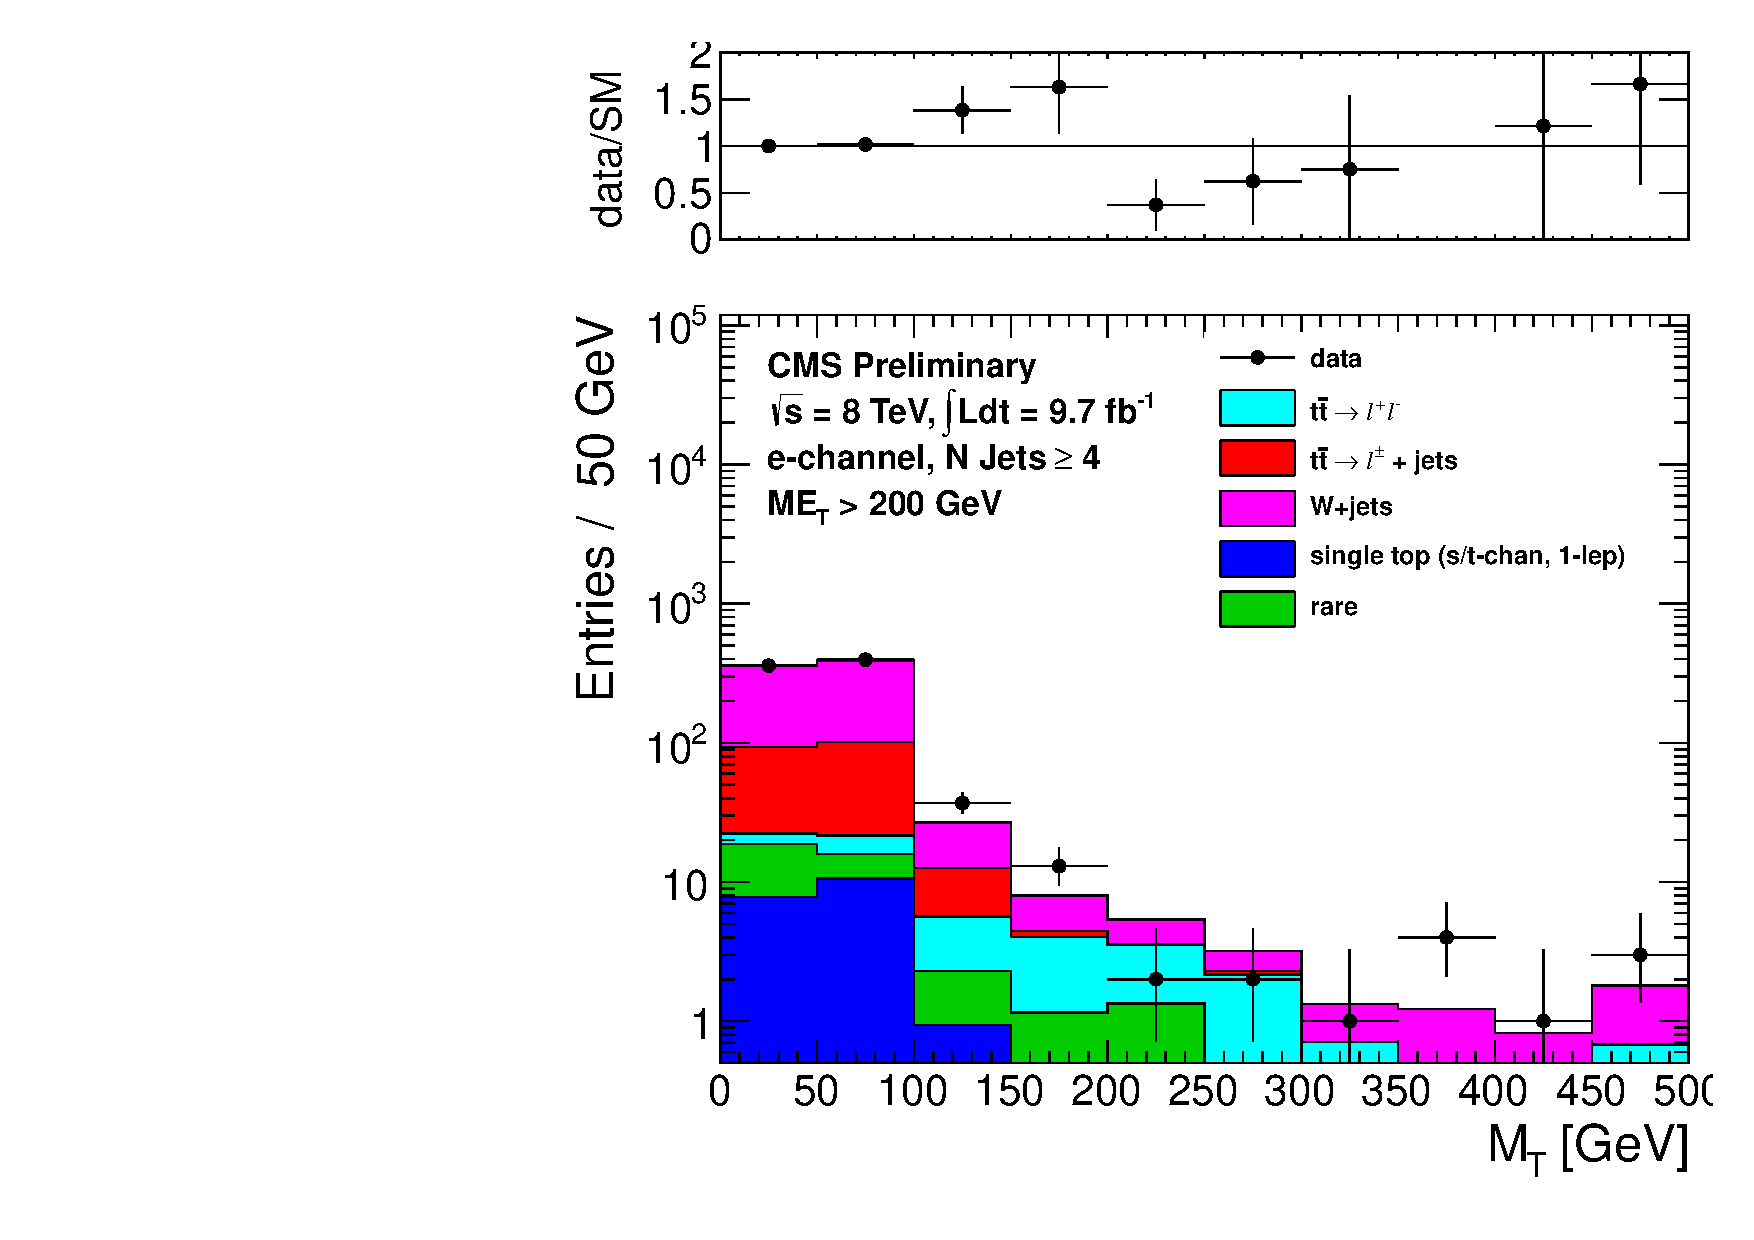
\includegraphics[width=0.5\linewidth]{plots/CR1plots/mt_met200_leadele_nj4.pdf}
	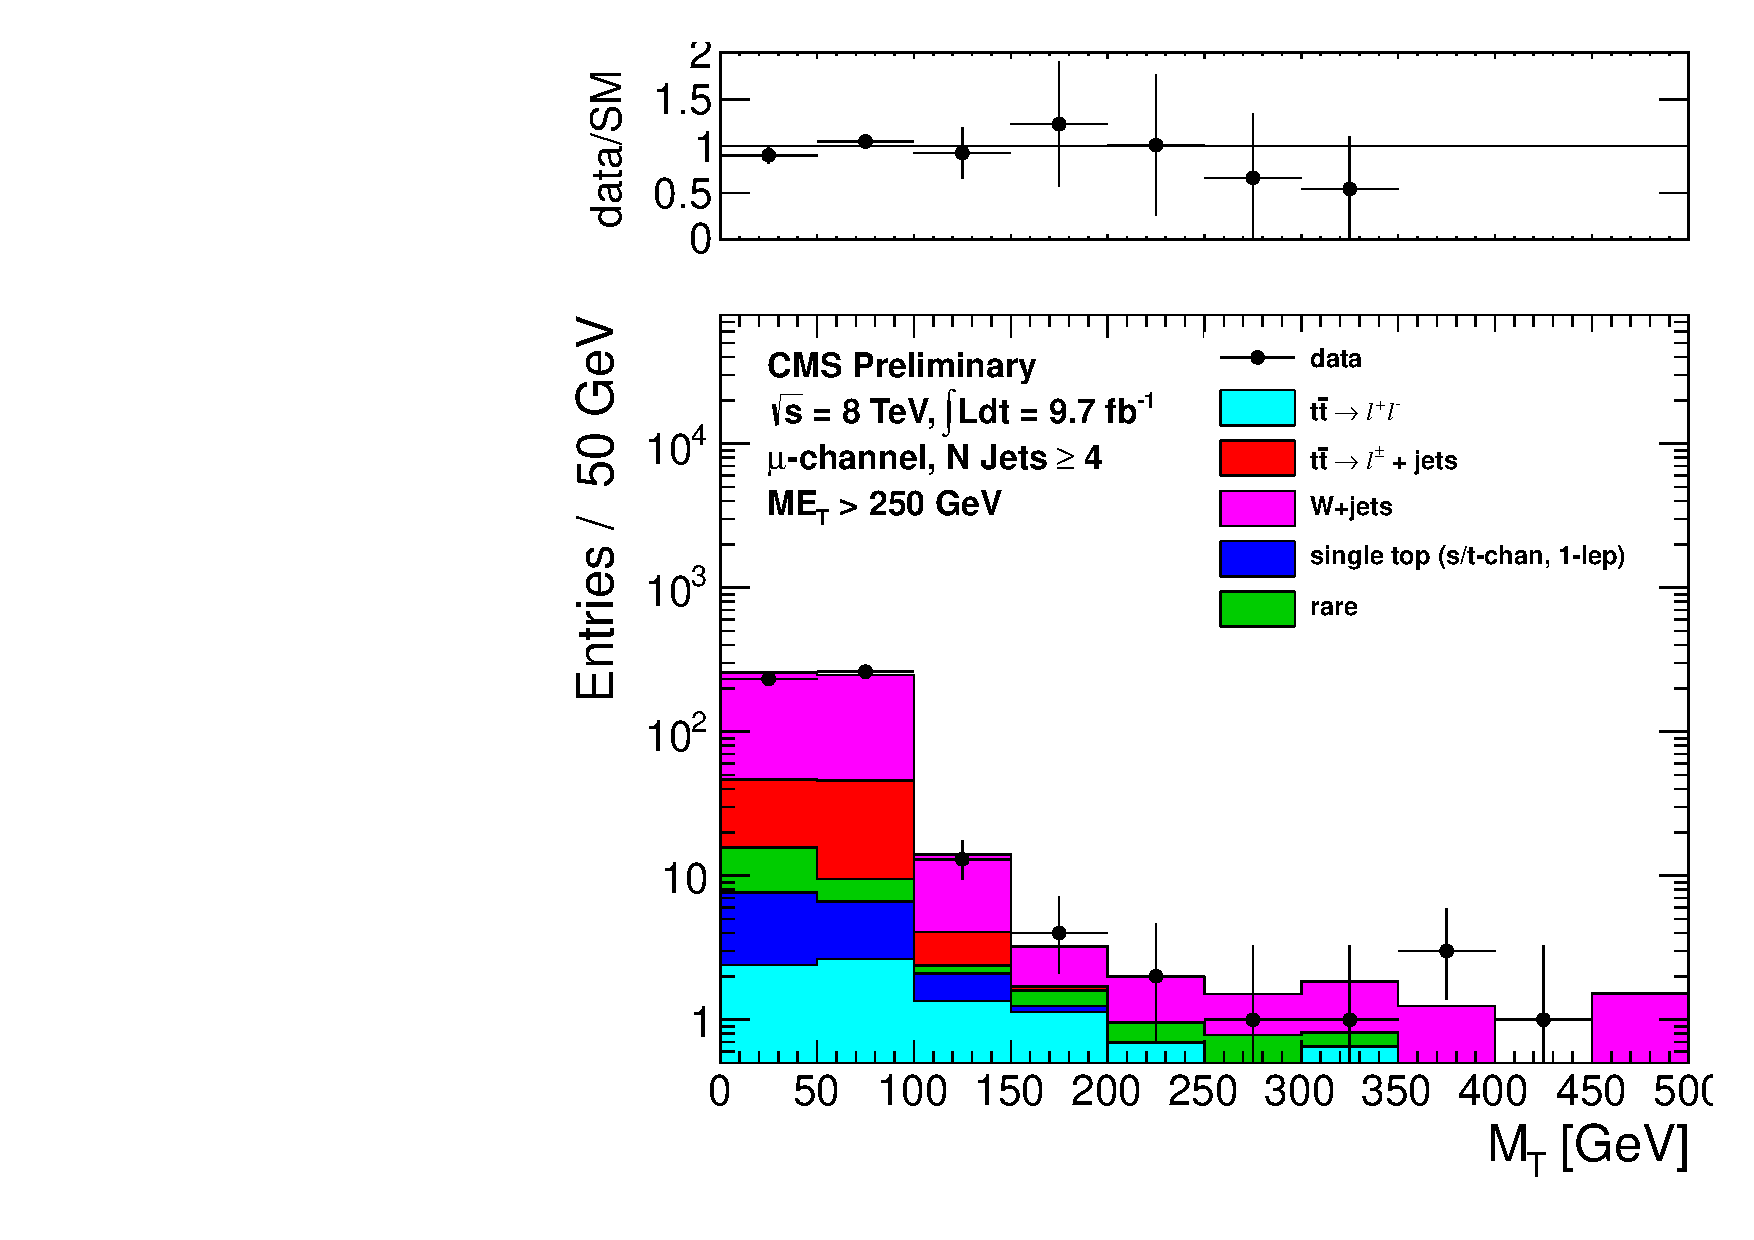
\includegraphics[width=0.5\linewidth]{plots/CR1plots/mt_met250_leadmuo_nj4.pdf}%
	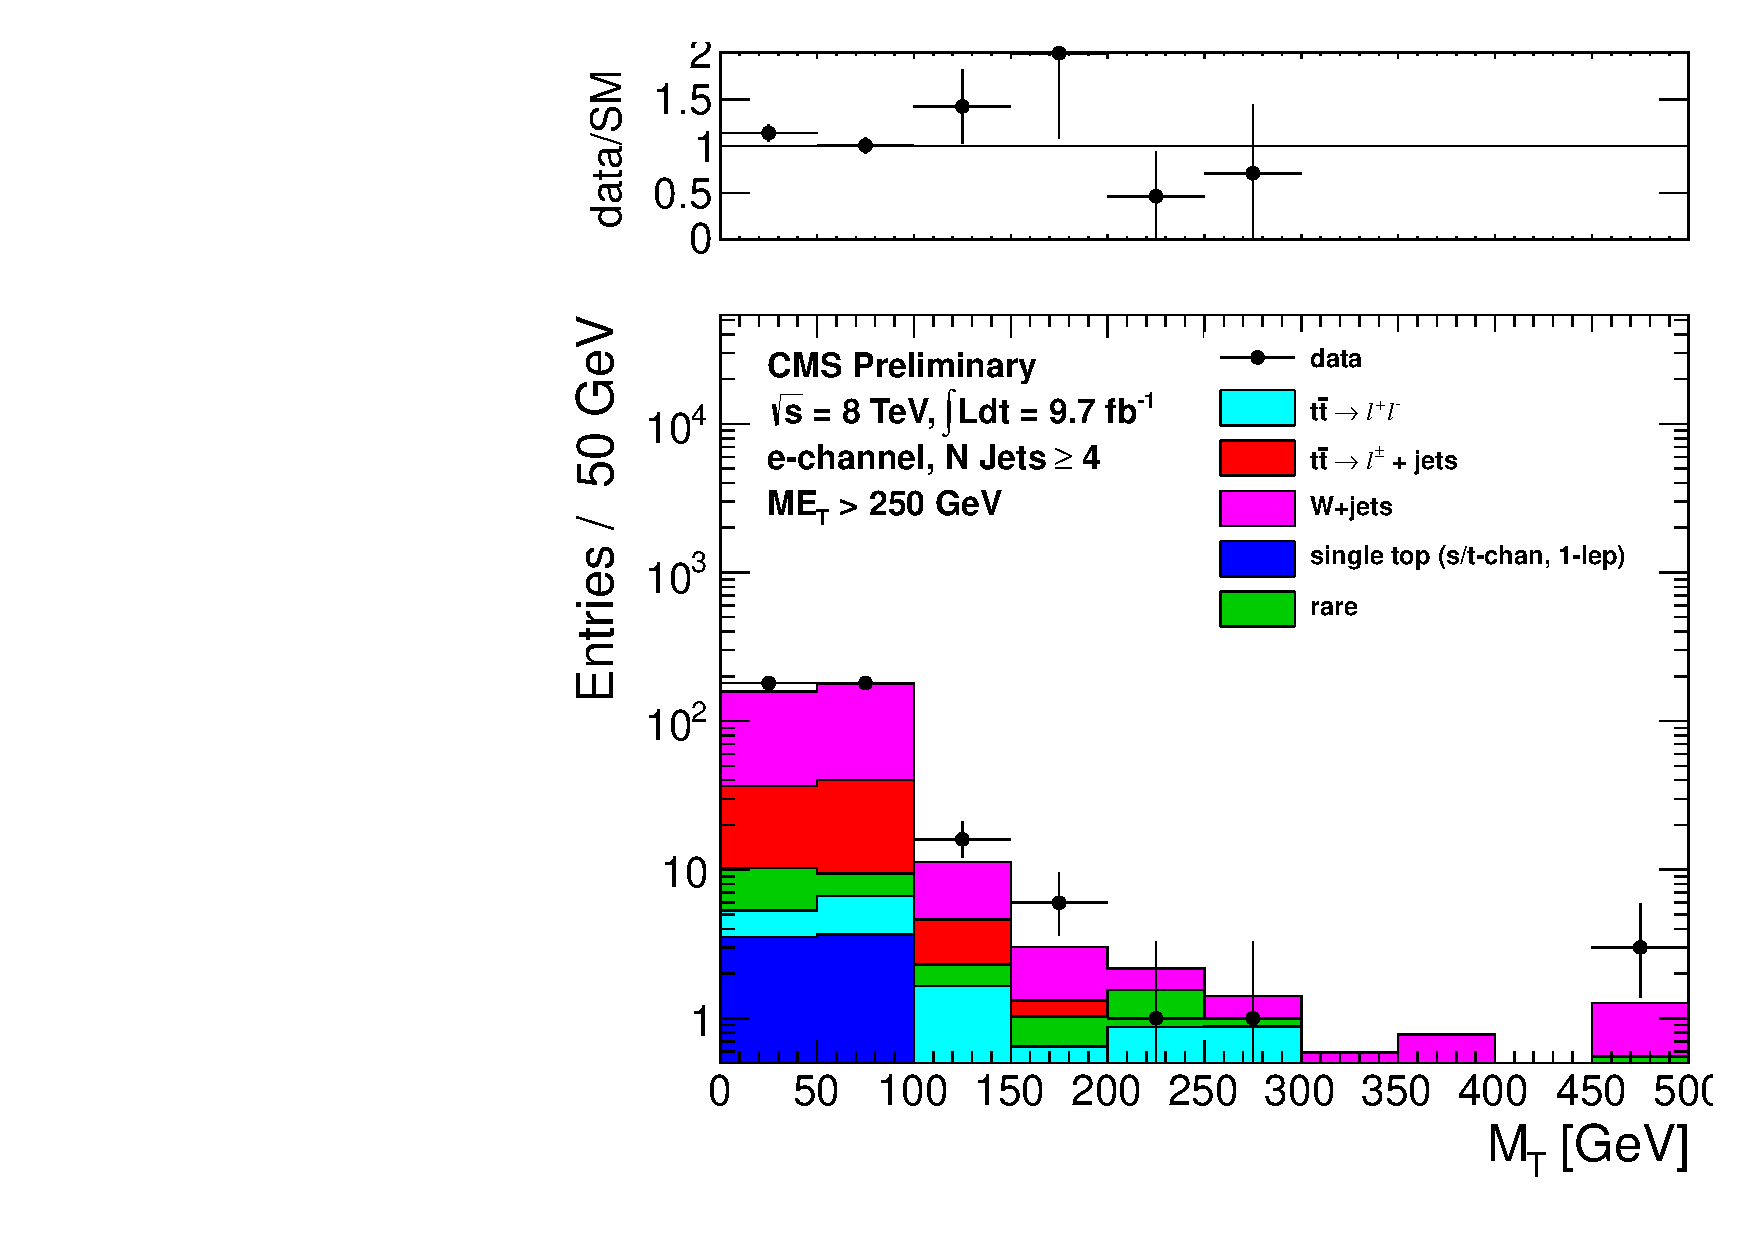
\includegraphics[width=0.5\linewidth]{plots/CR1plots/mt_met250_leadele_nj4.pdf}
    \caption{
      Comparison of the \mt\ distribution in data vs. MC for events
      with a leading muon (left) and leading electron (right)
      satisfying the requirements of CR1. The \met\ requirements used are
      150 GeV (top), 200 GeV (middle) and 250 GeV (bottom).
\label{fig:cr1mtrest} 
}  
      \end{center}
\end{figure}


\subsubsection{Single Lepton Top MC Modelling Validation}

The \mt\ tail for single-lepton top events (\ttsl\ and single top) is dominated by jet resolution effects. The \W\ cannot be far off-shell because $\mW < \mtop$.
The modeling of the \mt\ tail from jet resolution effects is studied using \zjets\ data and MC samples. 
\Z\ events are selection by requiring 2 good leptons (satisfying ID and isolation requirements) and requiring the \mll\ to be in the range $81-101$ GeV. 
The negative lepton is treated as a neutrino and so is added to the MET: \met\ $\rightarrow$ \pt(\Lepm) + \met, 
and the \mt\ is recalculated with the positive lepton \mt(\Lepp, \met).
The resulting ``pseudo-\mt'' is dominated by jet resolution effects, since no off-shell 
\Z\ production enters the sample due to the \mll\ requirement.
This section describes how well the MC predicts the tail of ``pseudo-\mt''. 



\begin{table}[!h]
\begin{center}
\begin{tabular}{l||c|c||c|c|c|c}
\hline
Sample              & CR2PRESEL0 &CR2PRESEL1 & CR2A & CR2B & CR2C & CR2D \\
\hline
\hline
DY MC 		  & $35 \pm 2$ & $30 \pm 2$ & $18 \pm 2$ & $32 \pm 3$ & $12 \pm 2$ & $5 \pm 1$ \\
Data - non-DY MC 	  & $65 \pm 9$ & $50 \pm 8$ & $36 \pm 6$ & $49 \pm 7$ & $25 \pm 5$ & $14 \pm 4$ \\
\hline
Data/MC SF 	  & $1.88 \pm 0.29$ & $1.68 \pm 0.30$ & $1.94 \pm 0.40$ & $1.54 \pm 0.29$ & $2.12 \pm 0.58$ & $2.96 \pm 1.22$ \\
\hline
\end{tabular}
\caption{ Yields in \mt\ tail comparing the MC prediction (after
  applying SFs) to data. CR2PRESEL refers to a sample with $\met>50$
  GeV and $\mt>150$ GeV.
  The uncertainties are statistical only.
\label{tab:cr2yields}}
\end{center}
\end{table}

\begin{figure}[hbt]
  \begin{center}
	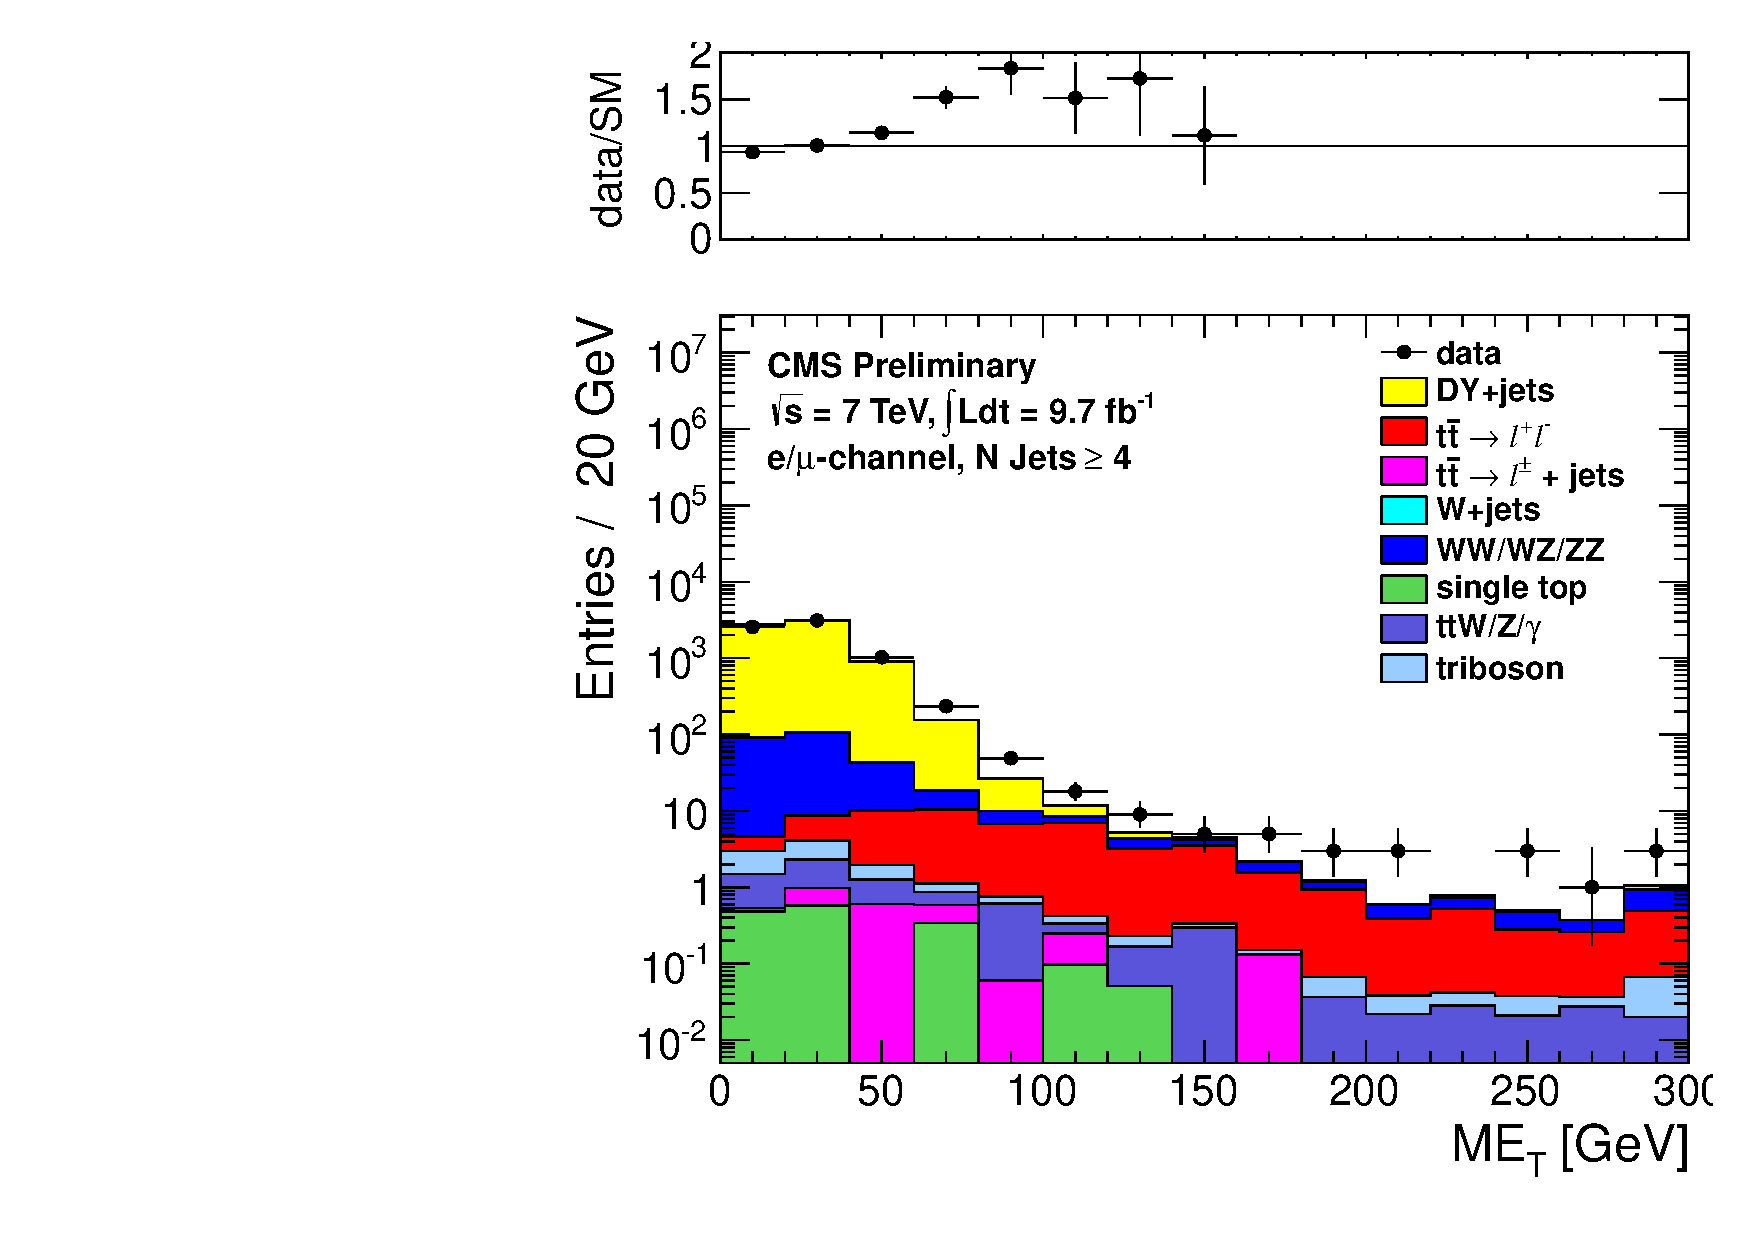
\includegraphics[width=0.5\linewidth]{plots/CR2plots/met_scaled_nj4_emucomb.pdf}%
	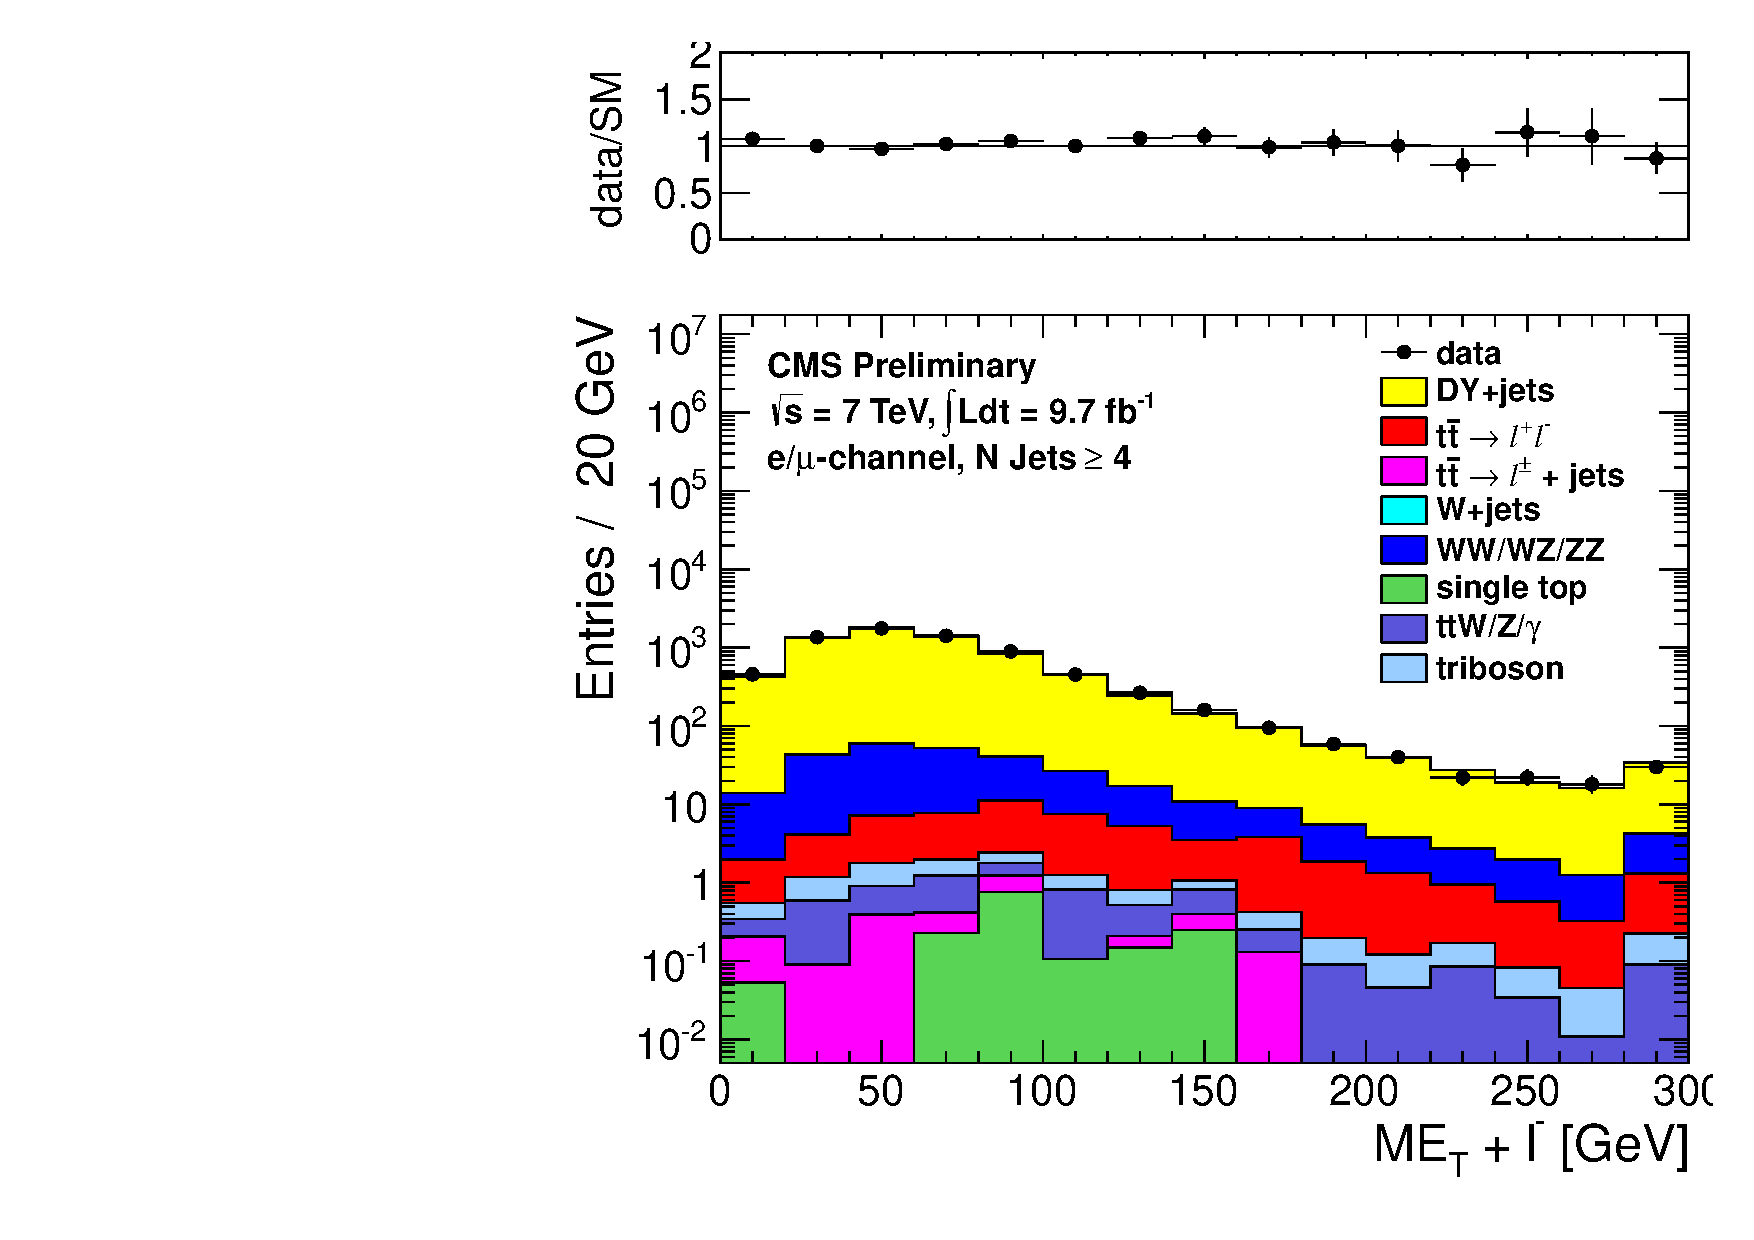
\includegraphics[width=0.5\linewidth]{plots/CR2plots/met_lepcor_scaled_nj4_emucomb.pdf}
	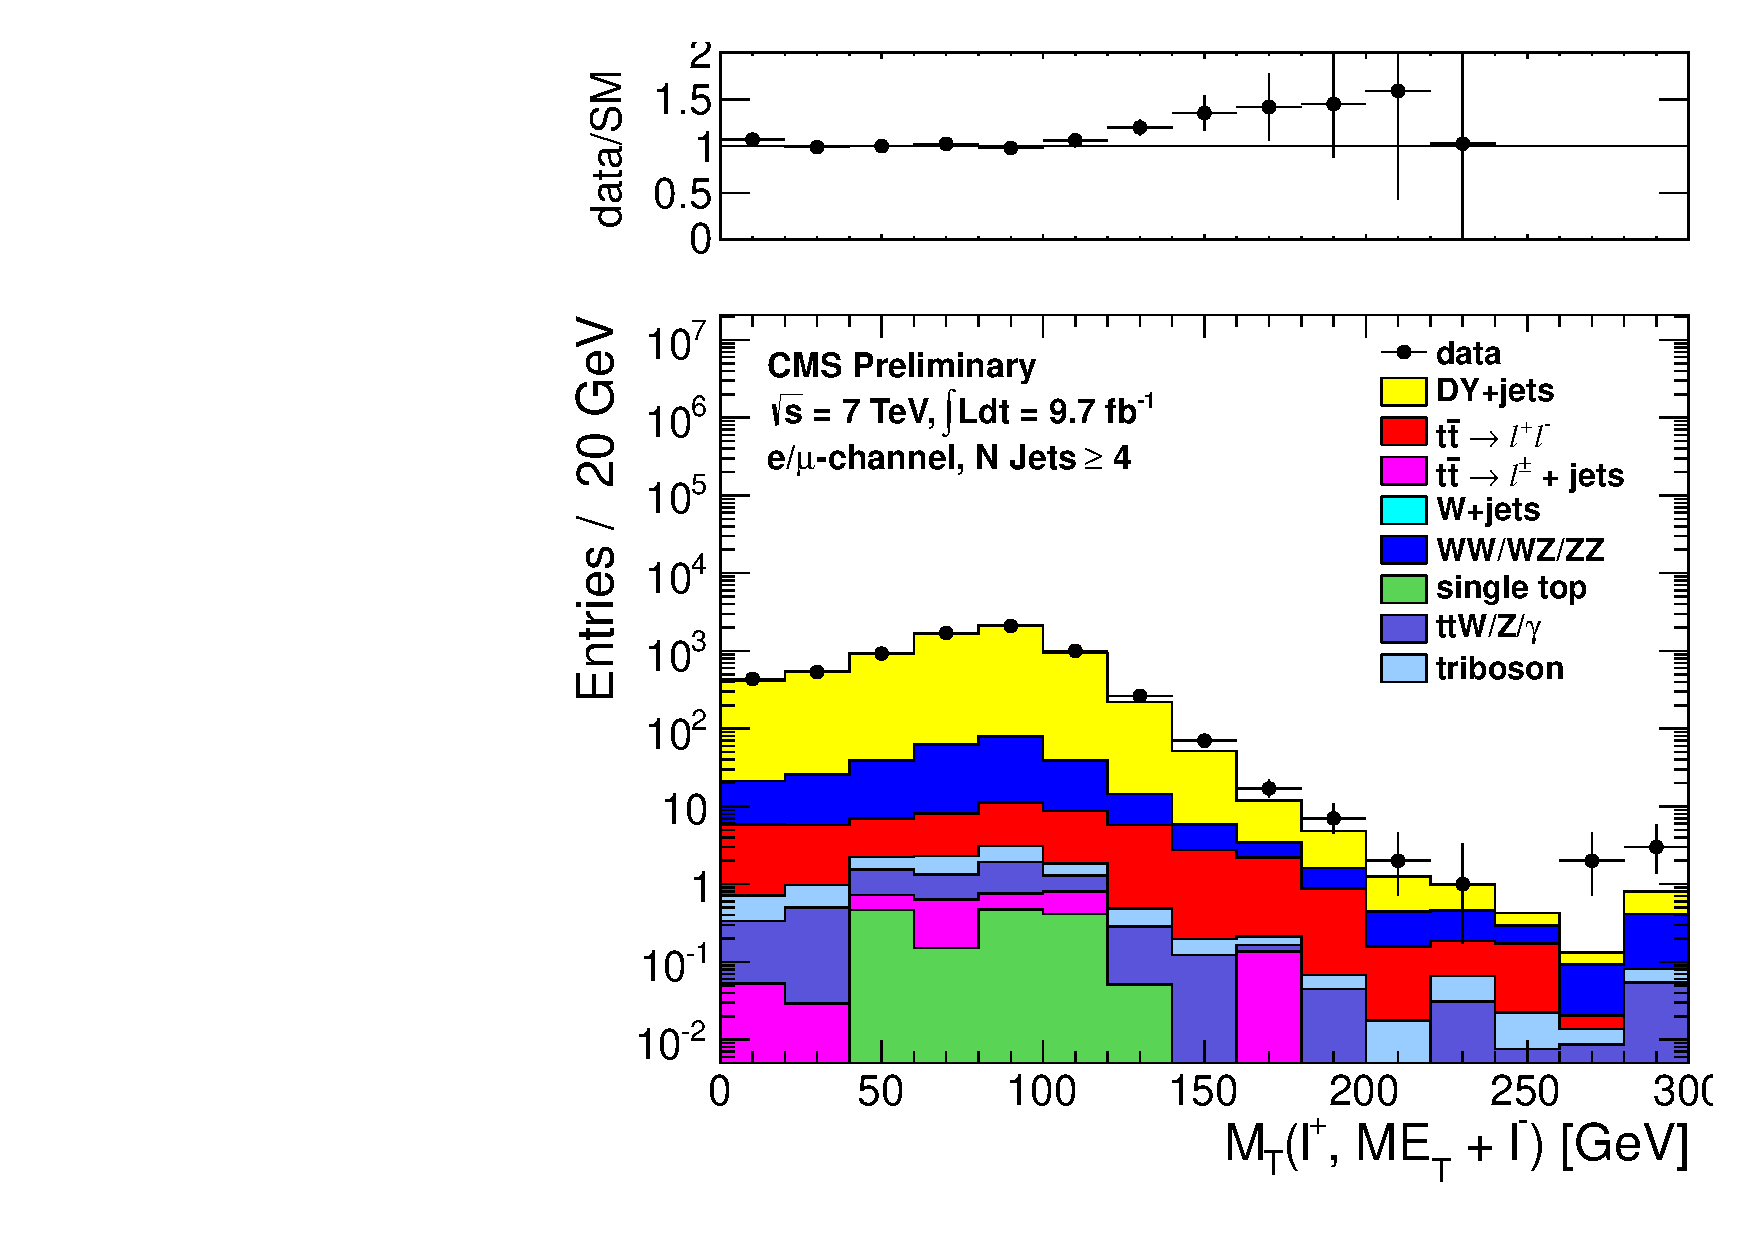
\includegraphics[width=0.5\linewidth]{plots/CR2plots/mt_lepcor_scaled_nj4_emucomb.pdf}%
	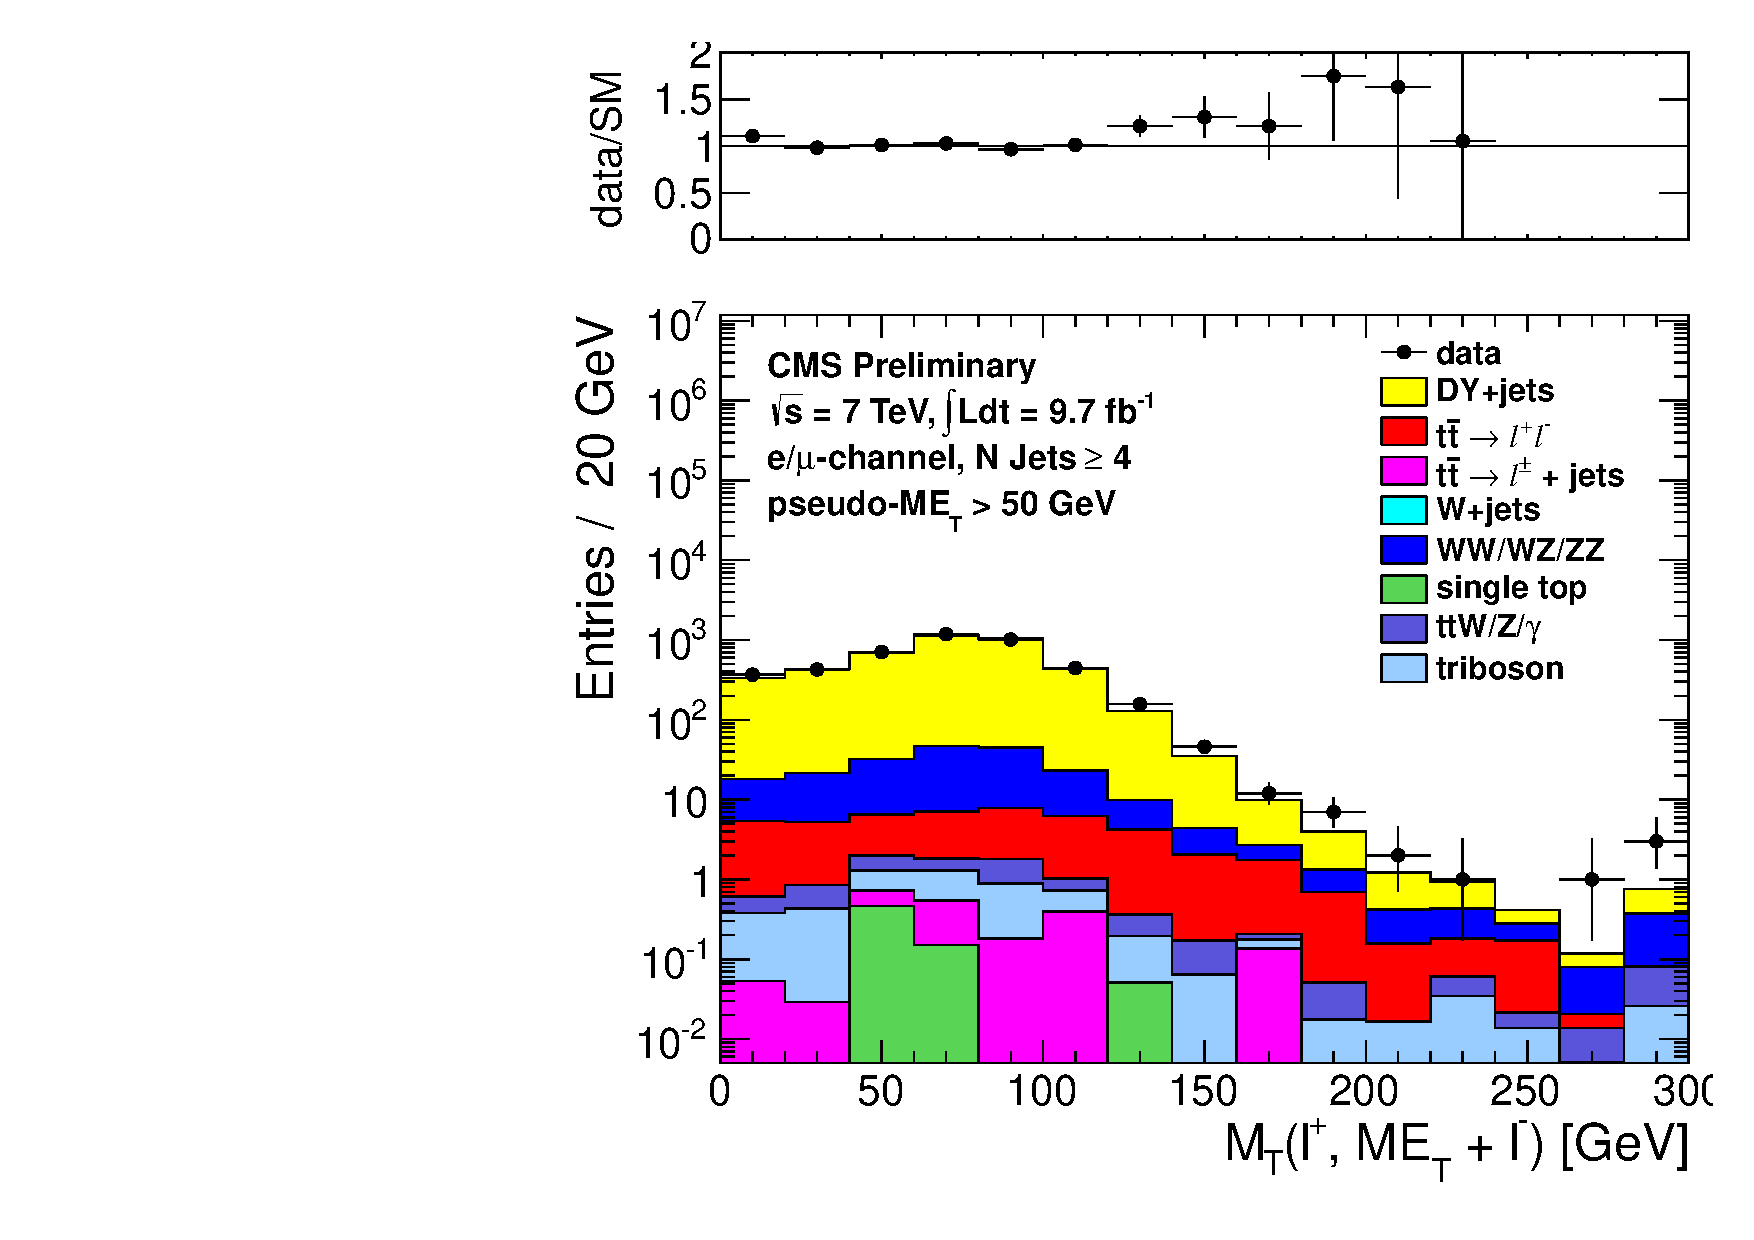
\includegraphics[width=0.5\linewidth]{plots/CR2plots/mt_lepcor_scaled_met50_nj4_emucomb.pdf}
    \caption{
      Comparison of the \met\ (top, left), pseudo-\met\ (top, right)
      and pseudo-\mt\ (bottom) distributions in data vs. MC for events
      satisfying the requirements of CR2, combining both the muon and
      electron channels. The pseudo-\mt\ distributions are shown
      before any additional requirements (bottom, left) and after
      requiring pseudo-\met>50 GeV (bottom, right).
\label{fig:cr2met} 
}  
      \end{center}
\end{figure}

\begin{figure}[hbt]
  \begin{center}
	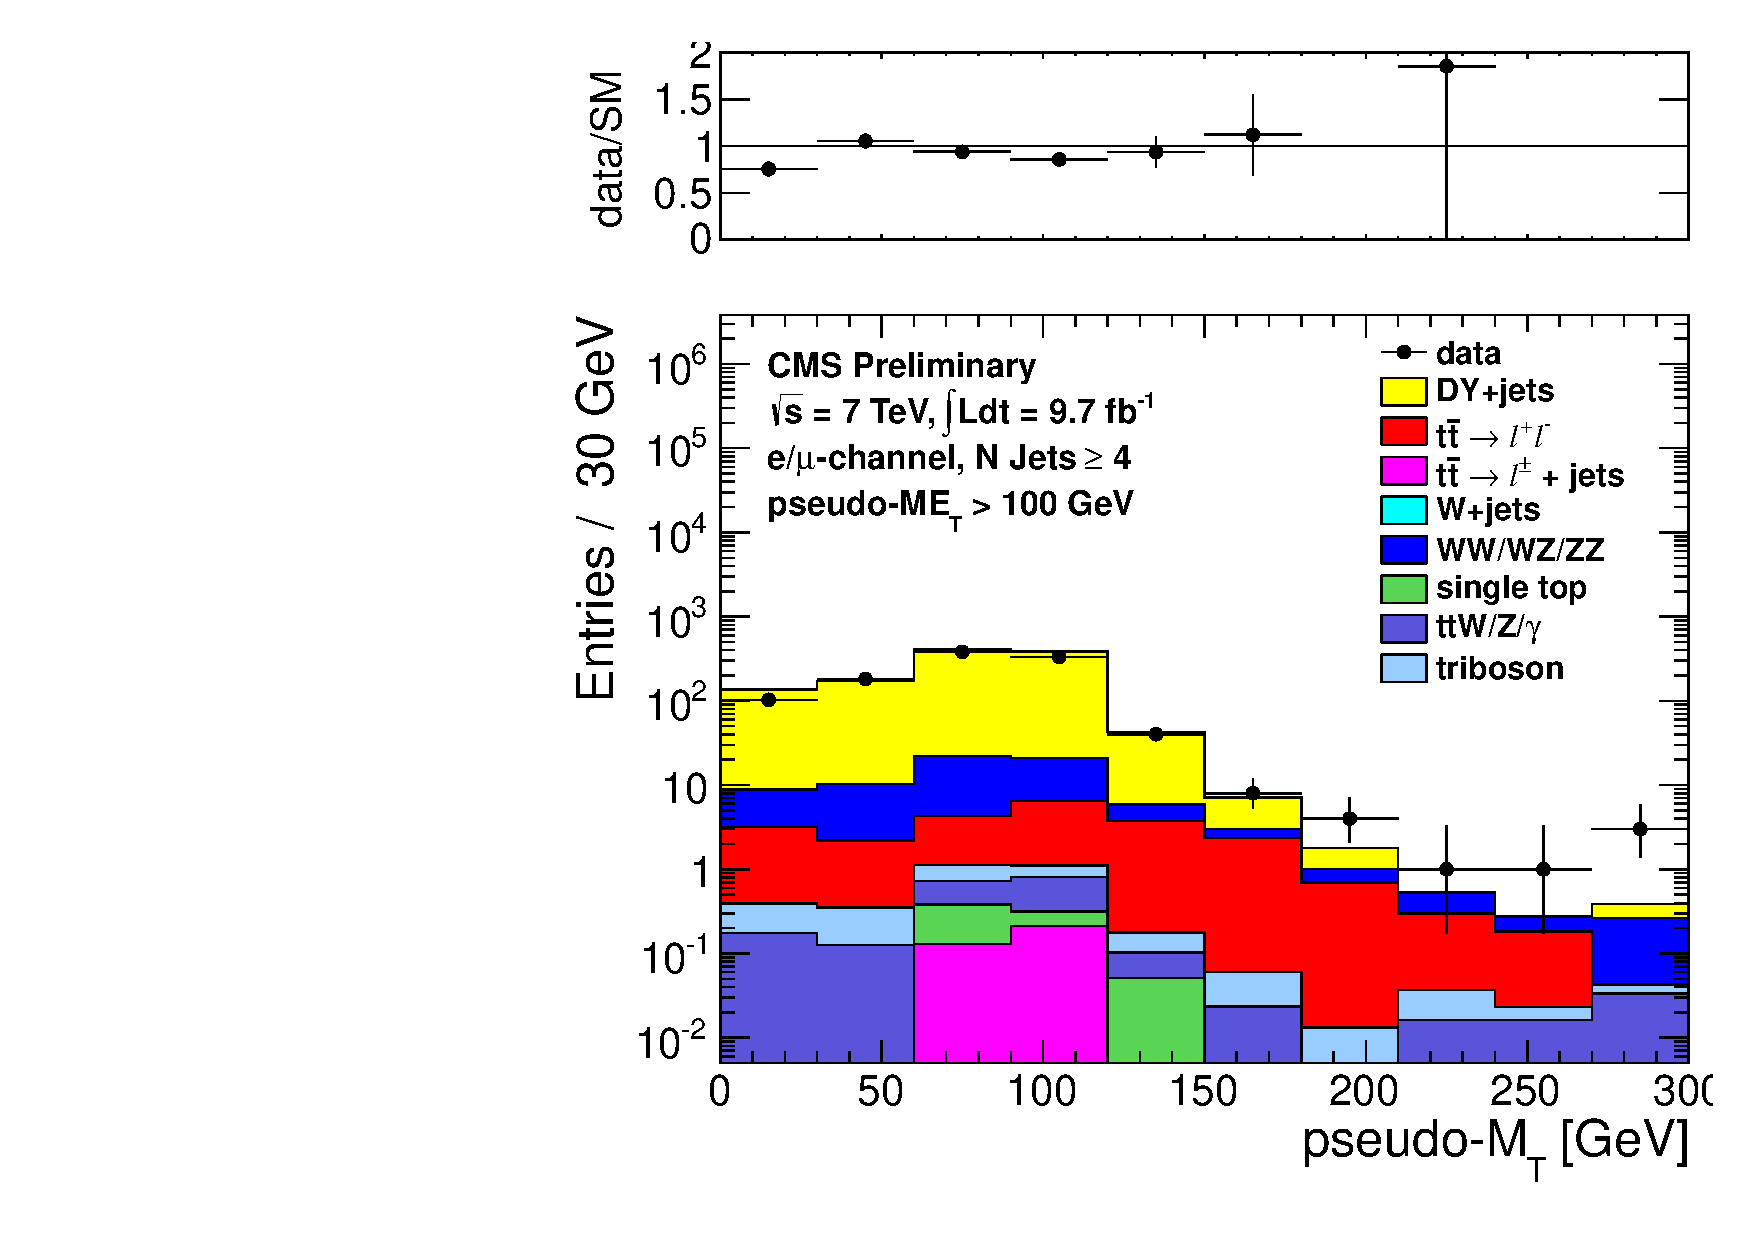
\includegraphics[width=0.5\linewidth]{plots/CR2plots/mt_lepcor_scaled_met100_nj4_emucomb.pdf}%
	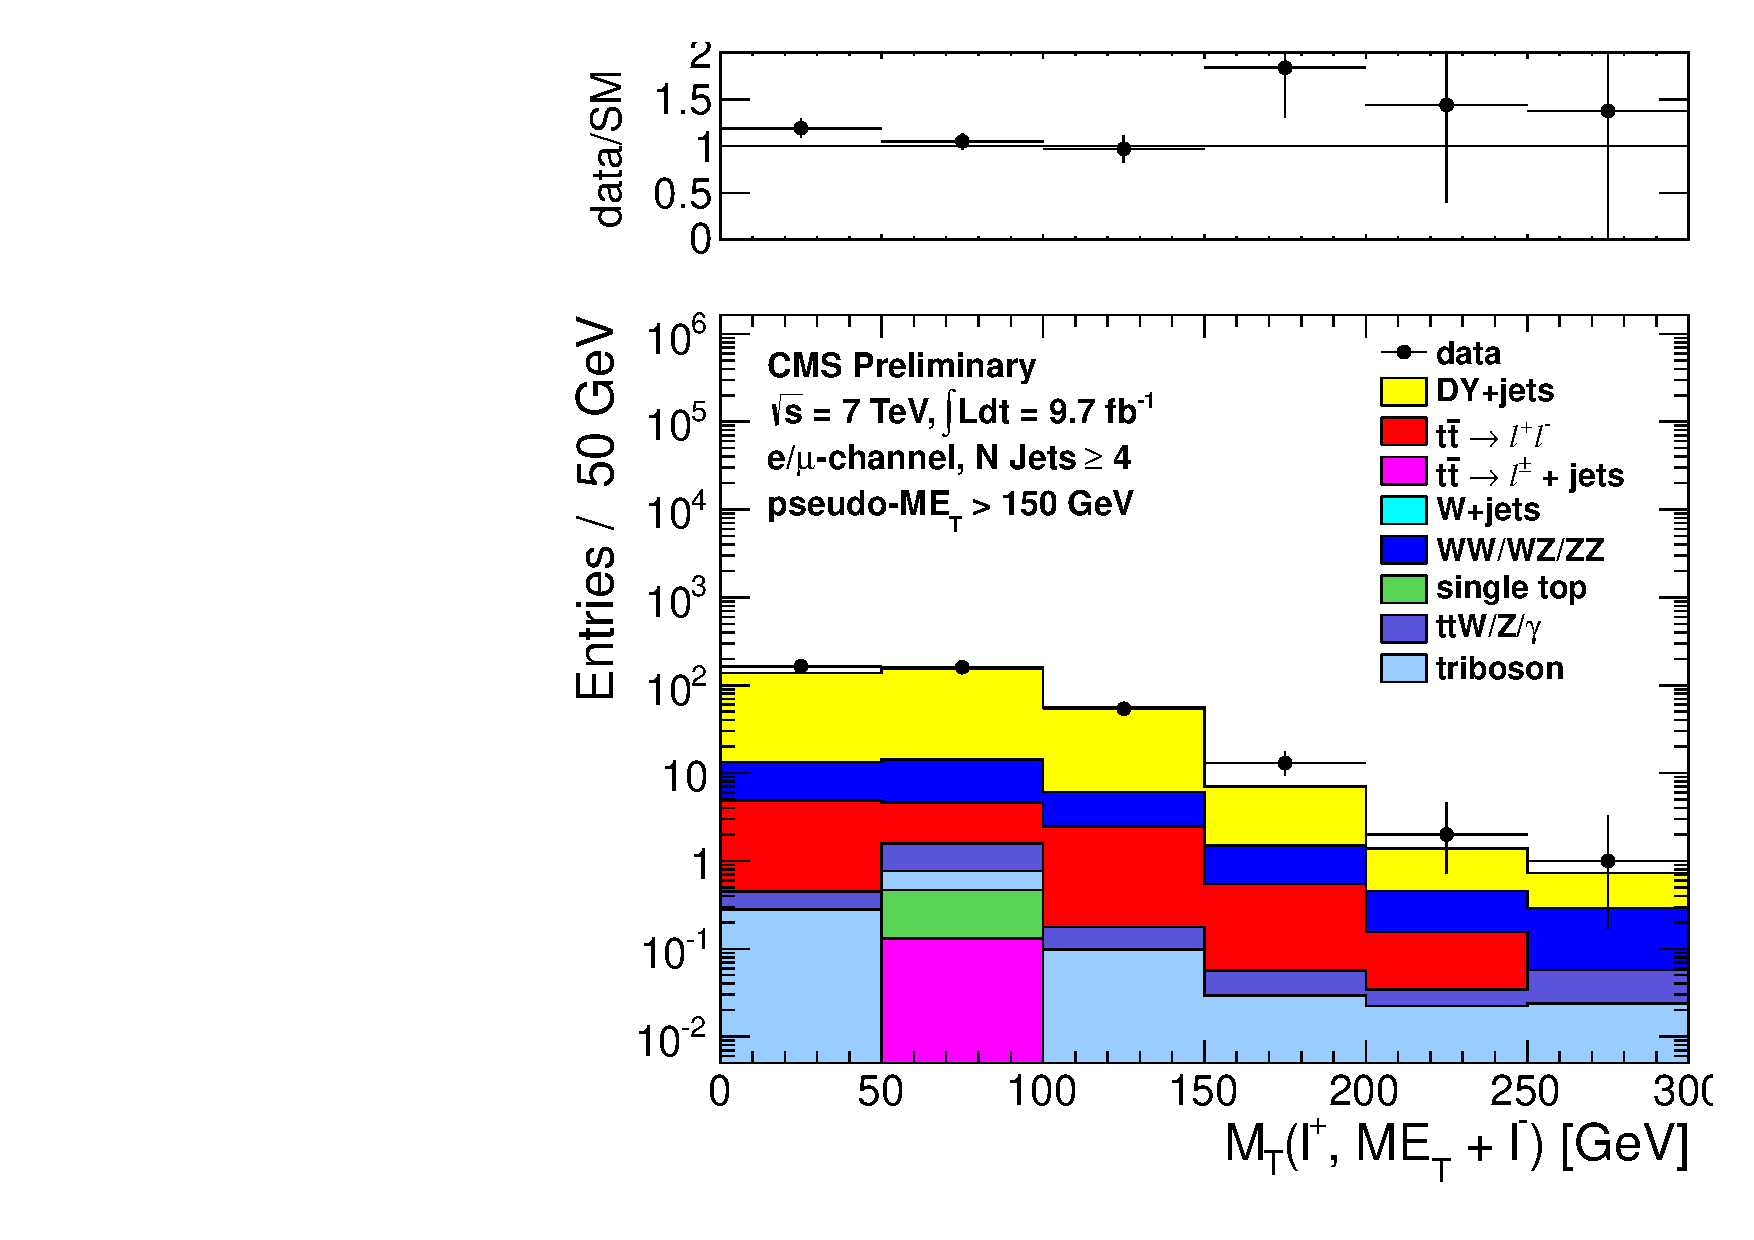
\includegraphics[width=0.5\linewidth]{plots/CR2plots/mt_lepcor_scaled_met150_nj4_emucomb.pdf}
	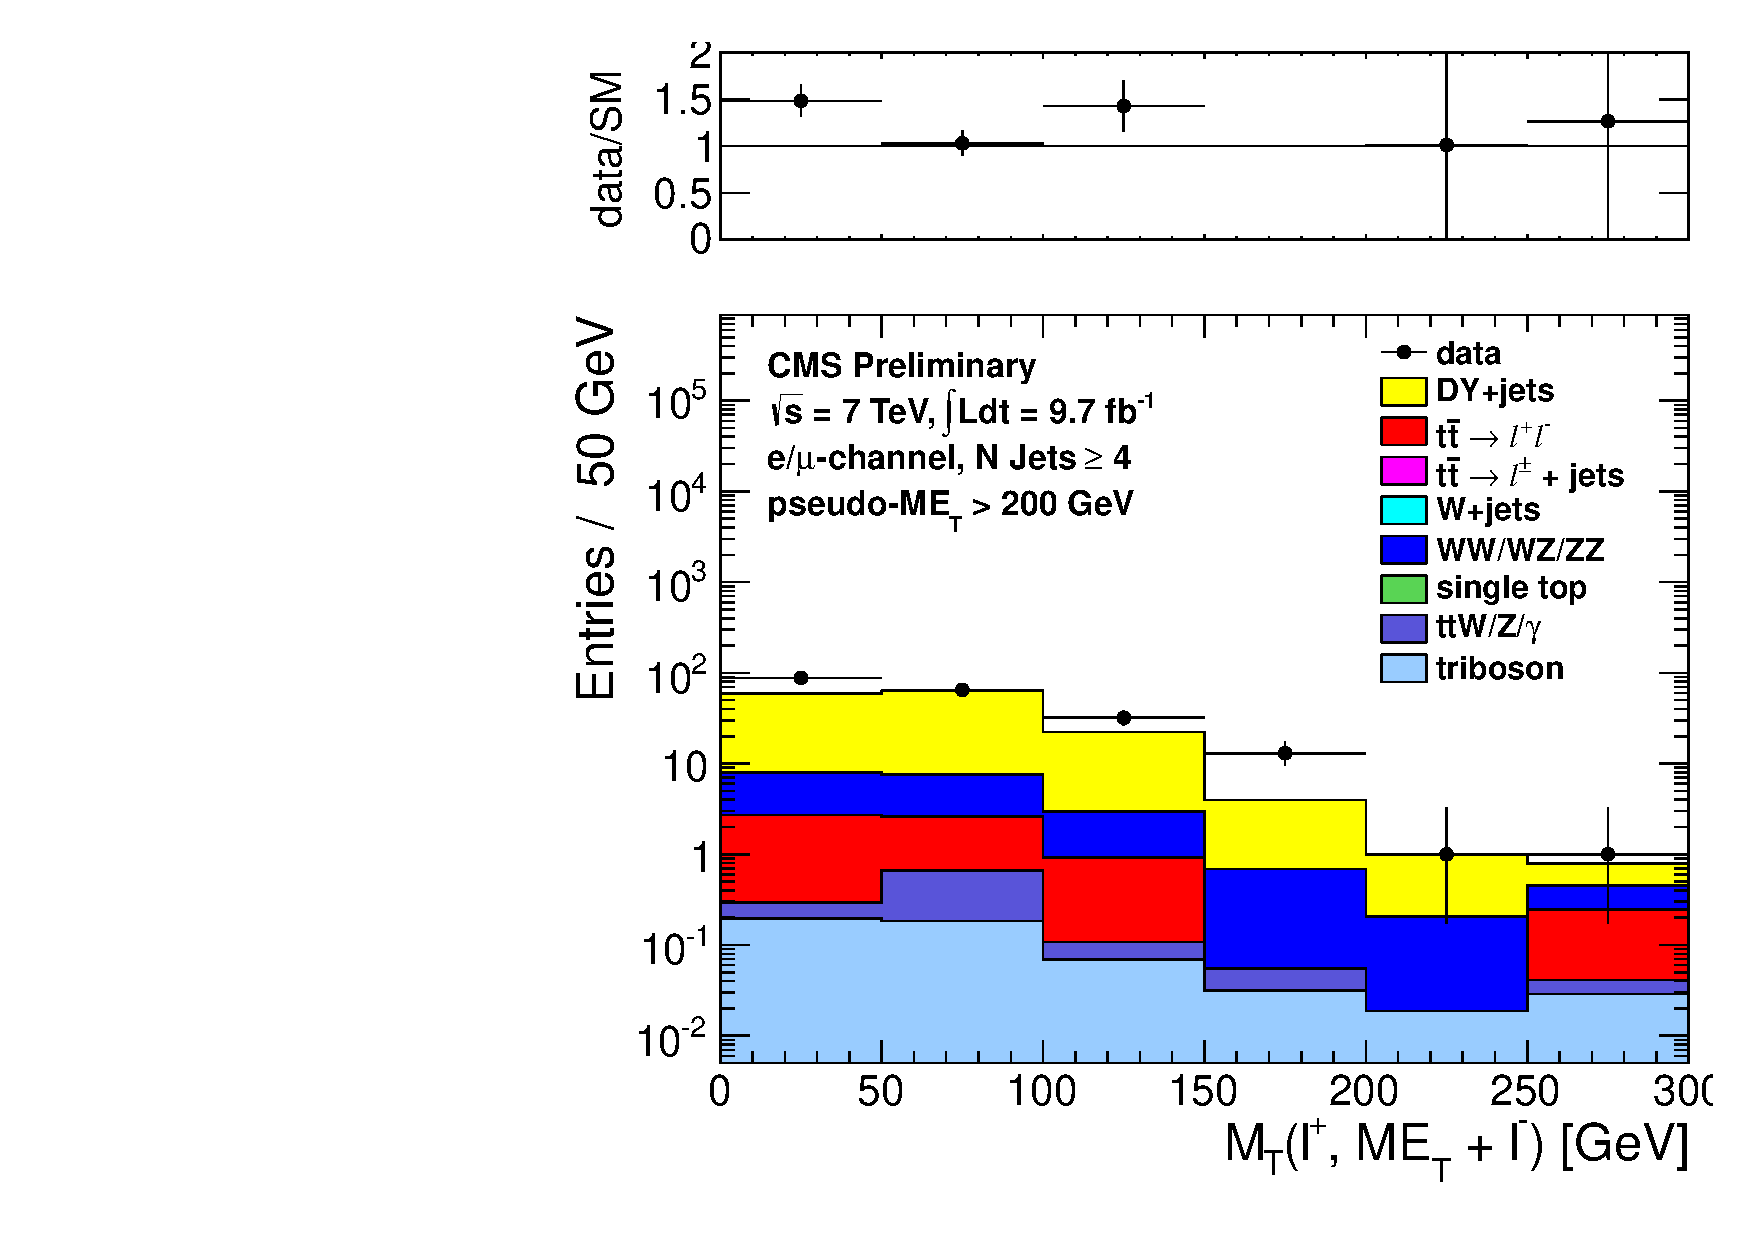
\includegraphics[width=0.5\linewidth]{plots/CR2plots/mt_lepcor_scaled_met200_nj4_emucomb.pdf}%
	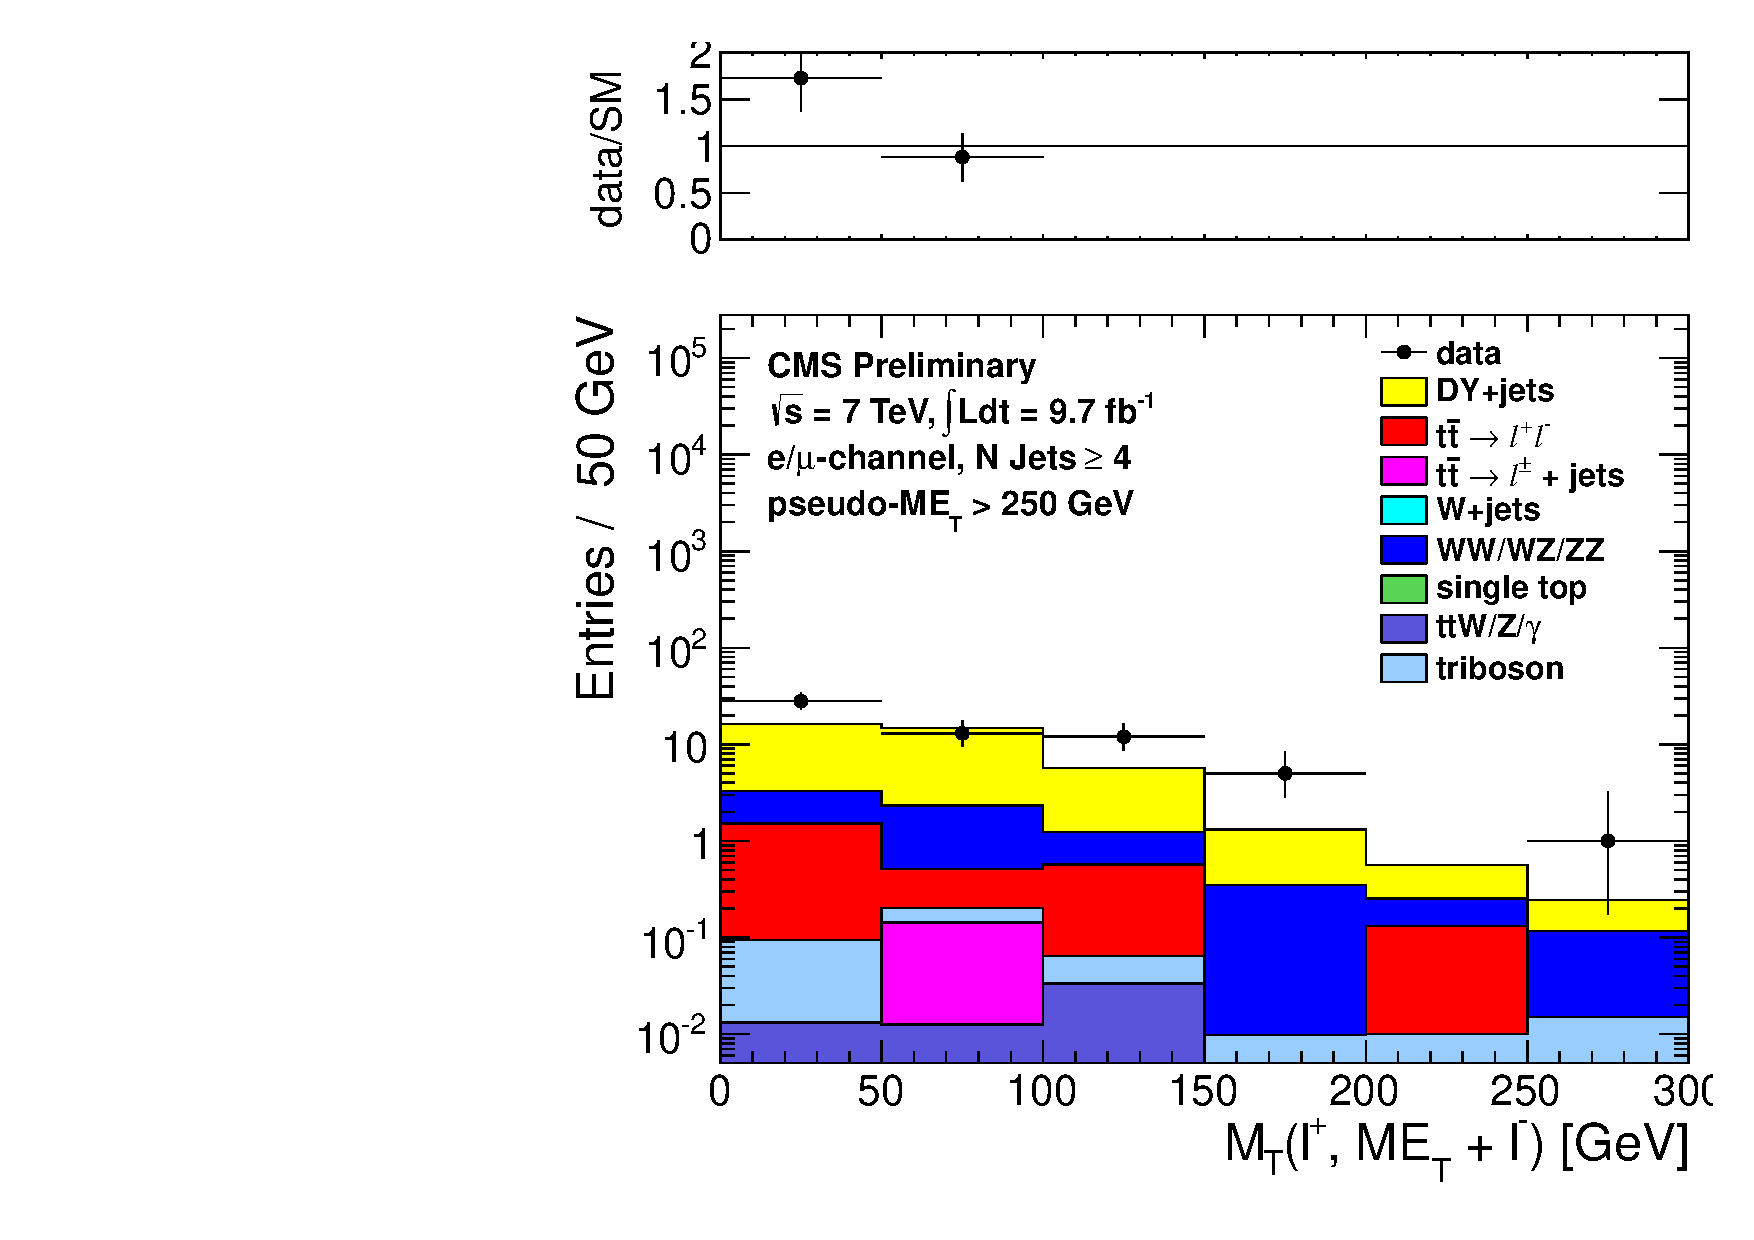
\includegraphics[width=0.5\linewidth]{plots/CR2plots/mt_lepcor_scaled_met250_nj4_emucomb.pdf}
    \caption{
      Comparison of the \mt\ distribution in data vs. MC for events
      satisfying the requirements of CR2, combining both the muon and
      electron channels. The pseudo-\met\ requirements used are
      100 GeV (top, left), 150 GeV (top, right), 200 GeV (bottom,
      left) and 250 GeV (bottom, right).
\label{fig:cr2mtrest} 
}  
      \end{center}
\end{figure}
